% ---------------------------------------------------------------------------
% Group 21 report: Formative Assignment 2 (NLP and Language Technologies).
% Build: tectonic main.tex   (or pdflatex + bibtex, or upload report/ and results/ to Overleaf)
% Figures and the main results table are read from ../results/, which notebooks
% 01-07 regenerate, so the report always shows the logged numbers.
% ---------------------------------------------------------------------------
\documentclass[conference]{IEEEtran}
\usepackage{iftex}
\ifXeTeX                       % Tectonic/XeLaTeX: a Times clone, as IEEEtran sets with pdfLaTeX
  \usepackage{amsmath,amssymb}
  \usepackage{unicode-math}
  \setmainfont{texgyretermes}[Extension=.otf, UprightFont=*-regular, BoldFont=*-bold,
                              ItalicFont=*-italic, BoldItalicFont=*-bolditalic]
  \setmathfont{texgyretermes-math.otf}
\else
  \usepackage{amsmath,amssymb}
\fi
\usepackage{booktabs}
\usepackage{graphicx}
\usepackage[table]{xcolor}
\usepackage{url}
\usepackage[hidelinks]{hyperref}
\usepackage{cite}
\graphicspath{{../results/}}

% ---- fill these in before submission ---------------------------------------
\newcommand{\MemberOne}{Hassan Adelani Luqman}
\newcommand{\MemberTwo}{Haguma Bianca}
\newcommand{\MemberThree}{Emmanuel Mukasa}
\newcommand{\MemberFour}{Emmanuel Nsabagasani}
\newcommand{\VideoLink}{\url{https://youtu.be/Gv1f1HYyZ18}}
\newcommand{\TrackerLink}{\url{https://docs.google.com/spreadsheets/d/1lV5C-49tpxNkssPY9lWKOiY321QZCv3a-YPMJONuf9E/edit?usp=sharing}}
\newcommand{\RepoLink}{\url{https://github.com/Hassan-Adelani-Luqman/nlp-sequential-modeling-group21}}
% ----------------------------------------------------------------------------

\begin{document}

\title{Does Order Matter? Sequential Models for\\Spoken Swahili Word Recognition}

\author{\IEEEauthorblockN{\MemberOne, \MemberTwo, \MemberThree, \MemberFour}
\IEEEauthorblockA{Group 21 \,$\cdot$\, NLP and Language Technologies, Formative Assignment 2}}

\maketitle

\begin{abstract}
Voice interfaces built on a handful of spoken words could serve users with limited literacy, but African languages
such as Swahili have little labelled speech. We ask how effectively sequential models recognise 12 spoken Swahili
words (the Zindi Swahili Audio Classification data, 4{,}200 clips), and what evidence supports their strengths and
limitations. Five approaches differ in how they model temporal order: order-free MFCC statistics with logistic
regression, a GMM-HMM, a BiLSTM with attention, a temporal convolutional network (TC-ResNet), and a fine-tuned
multilingual self-supervised Transformer (XLS-R). All five share one frozen split and protocol, and the test split was
used only after every configuration was frozen. The order-aware models reach 96--98\% test accuracy, against 79.5\%
for order-free statistics, and a stress test that reverses or shuffles each word shows that they rely on order. The
fine-tuned XLS-R is best (98.1\% accuracy, log loss 0.093), and more accurate than every other model under
Holm-corrected McNemar tests. With only 24 clips per word, it is about as accurate as the models trained from scratch
on 245. The HMM, BiLSTM and TC-ResNet tie on accuracy, and the convolutional model has the lowest log loss of the
three, at 150K parameters. Ten test clips defeat every order-aware model. Confident learning and an external
recogniser trace several of them to the data: a likely label error, words said in English, and crops that missed the
word.
\end{abstract}

\begin{IEEEkeywords}
Swahili, keyword spotting, sequence models, HMM, LSTM, temporal convolution, wav2vec 2.0, low-resource languages
\end{IEEEkeywords}

\noindent\fbox{\parbox{\dimexpr\linewidth-2\fboxsep-2\fboxrule\relax}{\small\raggedright
\textbf{Code and results:} \RepoLink\\
\textbf{Demo video:} \VideoLink\\
\textbf{Contribution tracker:} \TrackerLink}}

% ---------------------------------------------------------------------------
% Introduction (Section 1). Citation keys match report/references.bib.
% ---------------------------------------------------------------------------
\section{Introduction}
\label{sec:intro}

Spoken digits and a spoken ``yes'' or ``no'' are enough to run a mobile-money transfer, a health hotline or a
phone menu. For users with limited literacy, voice is often the only practical interface~\cite{doumbouya2021using}.
Swahili is widely spoken across East Africa. Yet it remains a low-resource language for speech technology: it has
only limited labelled data~\cite{joshi2020state}, and it was missing from the first releases of the largest open
crowdsourced speech corpus~\cite{ardila2020common}. Recognising a small Swahili vocabulary reliably, cheaply and
with honest confidence is therefore a useful problem in its own right, as well as a test of how well modern sequence
models transfer to an African language.

We study the Zindi Swahili Audio Classification challenge~\cite{zindi2021swahili}: 4{,}200 crowdsourced clips of
12 words, the digits \textit{moja} to \textit{kumi} (one to ten), \textit{ndio} (yes) and \textit{hapana} (no),
scored by log loss. A spoken word is a \emph{sequence} of acoustic frames, and its identity depends on the order of
its sounds. The vocabulary makes this concrete: \textit{sita} (six) and \textit{tisa} (nine) contain the same sounds
in a different order. Our research question is therefore:
\begin{quote}
  \emph{How effectively can sequential modelling approaches recognise spoken Swahili words, and what evidence
  supports the strengths and limitations of each approach?}
\end{quote}

We answer it with five approaches that differ in \emph{how} they model temporal order. A1 discards order: it is a
logistic regression on MFCC statistics. A2 models order with a Markov chain: a GMM-HMM per word. A3 uses
recurrence: a bidirectional LSTM with attention. A4 uses convolution over time: TC-ResNet. A5 uses self-attention
after multilingual self-supervised pretraining: a fine-tuned XLS-R. All five share one frozen data split, one feature
pipeline and one evaluation code base. They were tuned on validation only, in 55 logged development runs, and the
test split was used only after every configuration was frozen.

Our contributions are:
\begin{itemize}
  \item \emph{A controlled comparison of five ways of modelling order} on an African-language speech task. Neural
        models are trained with three seeds, and the test results carry bootstrap confidence intervals and
        Holm-corrected McNemar tests (Section~\ref{sec:results}).
  \item \emph{Direct evidence of how the models use order.} A temporal-order stress test reverses or shuffles each
        word. It shows that all order-aware models depend on order, but that the pretrained A5 relies mainly on
        order within about 100~ms (Section~\ref{sec:errors}).
  \item \emph{A data-size curve.} With only 24 training clips per word, the pretrained model is already about as
        accurate as the models trained from scratch on all 245.
  \item \emph{An error analysis without a human listener.} It combines confident learning with an external Swahili
        recogniser. The clips that defeat every order-aware model are far more often quiet, noisy or badly cropped,
        and include a likely label error and words said in English.
  \item \emph{An open, reproducible pipeline.} The notebooks rebuild every table and figure in this report from the
        logged runs and predictions.
\end{itemize}

Section~\ref{sec:related} reviews related work, Section~\ref{sec:data} the data, and Section~\ref{sec:method} the
methods and metrics. Section~\ref{sec:results} reports and discusses the results, Section~\ref{sec:errors} analyses
the errors and limitations, and Section~\ref{sec:conclusion} concludes.

% ---------------------------------------------------------------------------
% Related Work (Section 2) - drafted for M2 (keyword spotting, recurrence,
% attention, augmentation). M4 adds the self-supervised speech models and
% African/low-resource speech subsection. Citation keys match report/references.bib.
% ---------------------------------------------------------------------------
\section{Related Work}
\label{sec:related}

\subsection{From HMMs to neural keyword spotting}
Recognising a word from a small vocabulary is one of the oldest speech tasks. Classic systems pair a compact
spectral representation, the mel-frequency cepstrum, which outperformed other parametric representations for
word recognition~\cite{davis1980comparison}, with one hidden Markov model per word, trained by Baum--Welch
re-estimation and decoded by maximum likelihood~\cite{rabiner1989tutorial}. Our A1 and A2 baselines follow this
tradition. A1 keeps only order-free statistics of the cepstral frames, and A2 is the per-word left-to-right HMM.

The task became a standard benchmark with the Speech Commands dataset, which also proposed a reproducible way to
report keyword-spotting accuracy~\cite{warden2018speech}. Convolutional networks then replaced HMM and DNN
pipelines for small-footprint keyword spotting. Under fixed budgets on multiplications and parameters, they
reduced the false-reject rate by 27--44\% relative to a DNN~\cite{sainath2015convolutional}. Temporal
convolutions over the frames, arranged in a compact residual network (TC-ResNet), made keyword spotting fast
enough for real-time use on phones (a reported 385$\times$ speed-up) while surpassing the accuracy of the previous
state of the art on Speech Commands~\cite{choi2019temporal}. This is the design behind our A4.

\subsection{Recurrence and attention}
Recurrent networks model a sequence by carrying a hidden state from frame to frame. Long short-term memory (LSTM)
units keep the error signal constant through gated memory cells, and can learn dependencies across more than
1{,}000 time steps~\cite{hochreiter1997long}. Stacked, bidirectional LSTMs brought this to acoustic modelling,
reaching a 17.7\% phoneme error rate on TIMIT~\cite{graves2013speech}. Attention replaces a single summary
vector with a learned, soft search over positions~\cite{bahdanau2015neural}. For speech commands, de Andrade et
al.\ combined convolution, recurrence and attention in one model, reaching 94.1\% and 94.5\% accuracy on Speech
Commands V1 and V2 with only 202K parameters. They also used the attention weights to show which parts of the
audio drove each decision~\cite{deandrade2018neural}.

Our A3 belongs to this line. It differs in separating the contributions: A3 is recurrent by default, the
convolutional front-end is tested as an ablation, and A4 is purely convolutional.

Whether recurrence is needed at all is itself an open question. A systematic comparison across sequence-modelling
benchmarks found that a simple convolutional architecture outperforms canonical recurrent networks such as LSTMs,
while also showing a longer effective memory~\cite{bai2018empirical}. Our A3--A4 comparison tests whether this
holds for sequences as short as a single spoken word, with only a few hundred training examples per class.

\subsection{Augmentation for small speech datasets}
SpecAugment showed that simple transformations applied directly to filter-bank features (time warping, and
masking blocks of frequency channels and of time steps) are enough to reach state-of-the-art results on large
speech-recognition benchmarks~\cite{park2019specaugment}. Our setting is the opposite extreme: about 245 training
clips per word, and competition rules that forbid external data such as noise corpora. Synthetic, feature-level
augmentation is therefore the only augmentation available to us, and its value is tested directly in round R2.

\subsection{Self-supervised speech models and African languages}
[M4: wav2vec~2.0 / XLS-R / MMS pretraining and fine-tuning; Common Voice; keyword spotting and speech technology
for African and other low-resource languages; the gap this study addresses.]

\subsection{How the literature shaped our study}
Three lessons from this work shaped the design:
\begin{enumerate}
  \item Keyword spotting has been solved with very different ways of modelling time: order-free features,
        Markov states, convolution, recurrence and self-attention. We therefore compare one representative of
        each on the same data, split and metrics, rather than tuning a single family.
  \item Attention-based recognisers can show where in the audio they look~\cite{deandrade2018neural}. We use this
        to test our central hypothesis directly: words whose sounds differ mainly in order (\textit{tisa} and
        \textit{sita}) should separate order-aware from order-free models.
  \item Augmentation such as SpecAugment is most useful when data is scarce~\cite{park2019specaugment}. With 245
        clips per word, we treat it as a first-class experimental factor rather than a fixed default.
\end{enumerate}

% ---------------------------------------------------------------------------
% Dataset and Exploratory Analysis (Section 3) - drafted for M3 (with M1's Phase 1 profiling).
% Numbers come from notebooks/01_eda.ipynb and results/metrics/; figures are
% results/figures/*.png (main.tex sets \graphicspath to ../results/).
% Needs in the preamble: \usepackage{booktabs, graphicx}.
% ---------------------------------------------------------------------------
\section{Dataset and Exploratory Analysis}
\label{sec:data}

\subsection{Data}
We use the Swahili Audio Classification dataset~\cite{zindi2021swahili}. It holds recordings of 12 spoken Swahili
words, made by about 300 crowd-workers in Kenya: the digits \textit{moja} to \textit{kumi} (one to ten),
\textit{ndio} (yes) and \textit{hapana} (no). There are 4{,}200 labelled clips, exactly 350 per word, and
1{,}800 unlabelled competition test clips. All 6{,}000 files are 16~kHz mono 16-bit PCM, with no corrupt files
and no byte-identical duplicates. The competition allows no external data and forbids redistribution, so the audio
is kept off the public repository. As described in Section~\ref{sec:method}, we froze one stratified 70/15/15
split (2{,}940 / 630 / 630 clips). The distribution statistics below use the training split only. Analyses that
score a model (the confusions, the prefix curve and the normalisation check) use the validation split, as model
selection does. None uses the test split.

\subsection{What the data revealed}
\paragraph{The words are short, but the clips are long}
Clips last 2.5--62~s (median 4.3~s), while the spoken word lasts a median 0.55~s. Word duration ranges from
0.45~s for \textit{tatu} to 0.65~s for the three-syllable \textit{hapana}, and 89.5\% of words last at most 1.0~s
(Fig.~\ref{fig:durations}). A 30~dB silence trim leaves a median of 1.9~s and a 95th percentile of 5.5~s,
because background noise is kept as part of the ``word''. The models therefore read a centred window around the
clip's highest-energy region: 1.5~s by default, 1.0~s for the final A3 and 2.0~s for the final A4. The 1.5~s window
retains a median 99.8\% of each clip's above-noise energy.

\paragraph{Recordings vary in level, but are mostly clean}
Levels span about 19~dB between the 5th and 95th percentiles (median $-32$~dBFS), and 3.8\% of clips reach full
scale, so windows are peak-normalised. The median estimated SNR is 42~dB, and 80\% of clips exceed 30~dB. Our
synthetic noise augmentation (10--30~dB) is therefore harsher than most real recordings. The noisy minority matters,
however: the models fail most on clips below 30~dB (Section~\ref{sec:errors}).

\paragraph{The vocabulary contains an anagram}
\textit{sita} (six) and \textit{tisa} (nine) contain the same sounds in a different order. The average
spectrograms show it directly (Fig.~\ref{fig:spectra}): the high-frequency energy of /s/ comes at the start of
\textit{sita} and in the middle of \textit{tisa}. Other near-pairs are \textit{nne}/\textit{nane} (letter edit
distance 1), and \textit{tano}/\textit{tatu} and \textit{saba}/\textit{sita} (distance 2). We track these four
pairs for every model. Spelling similarity, however, only weakly predicts what an order-free model confuses
(Spearman $\rho=-0.18$ over all 66 pairs, $p=0.16$). Its most confused pair on validation, \textit{mbili}/\textit{ndio}, is far
apart in spelling, but both words begin with a prenasalised stop and contain /i/.

\paragraph{Order-free features do not separate the words}
A t-SNE map of order-free MFCC statistics shows no word forming its own cluster. The only distinct islands contain
clips of many words, so they probably group recordings by speaker or recording condition. This is consistent with
the order-free baseline's ceiling of 77.9\%, and with the large gain from per-utterance normalisation in the HMM
(53\% to 76\% accuracy).

\paragraph{The evidence builds up through the word}
Trained on only the first 25/50/75/100\% of each word, the order-free classifier reaches 49/72/80/80\% accuracy.
Words that share a first syllable (\textit{tano}, \textit{tatu}) separate only once their second syllable begins.
The evidence therefore builds up over most of the word, not just its onset, and the window must cover the whole
word.

\paragraph{No leakage, but speakers are unknown}
No pair of clips across the splits is a near-duplicate (the maximum cosine similarity of standardised MFCC
statistics is 0.94). Median pitch spans 106--235~Hz between the 10th and 90th percentiles, consistent with a mix of
adult male and female voices. Speaker identities are not provided, however, so the same speaker may appear in
both training and test clips (Section~\ref{sec:limitations}).

\begin{table}[t]
  \centering
  \caption{How the exploratory analysis shaped the design.}
  \label{tab:eda}
  \small
  \begin{tabular}{@{}p{0.47\linewidth}p{0.45\linewidth}@{}}
    \toprule
    Finding & Decision \\
    \midrule
    350 clips per word, perfectly balanced & No class weighting; accuracy, macro-F1 and log loss \\
    Words last a median 0.55~s in 2.5--62~s clips; silence trimming leaves noisy tails & Centred 1.5~s energy window; 1.0/2.0~s tested \\
    Levels vary by $\sim$19~dB; median SNR 42~dB & Peak normalisation; CMVN for the HMM \\
    \textit{sita}/\textit{tisa} differ only in where /s/ occurs & Sequence models; four sound-alike pairs tracked \\
    Order-free features do not cluster by word & Per-utterance normalisation; order-aware models \\
    Evidence arrives through the word & Models see the whole word \\
    No near-duplicates; no speaker IDs & No leakage found; speaker overlap is a limitation \\
    \bottomrule
  \end{tabular}
\end{table}

\begin{figure}[t]
  \centering
  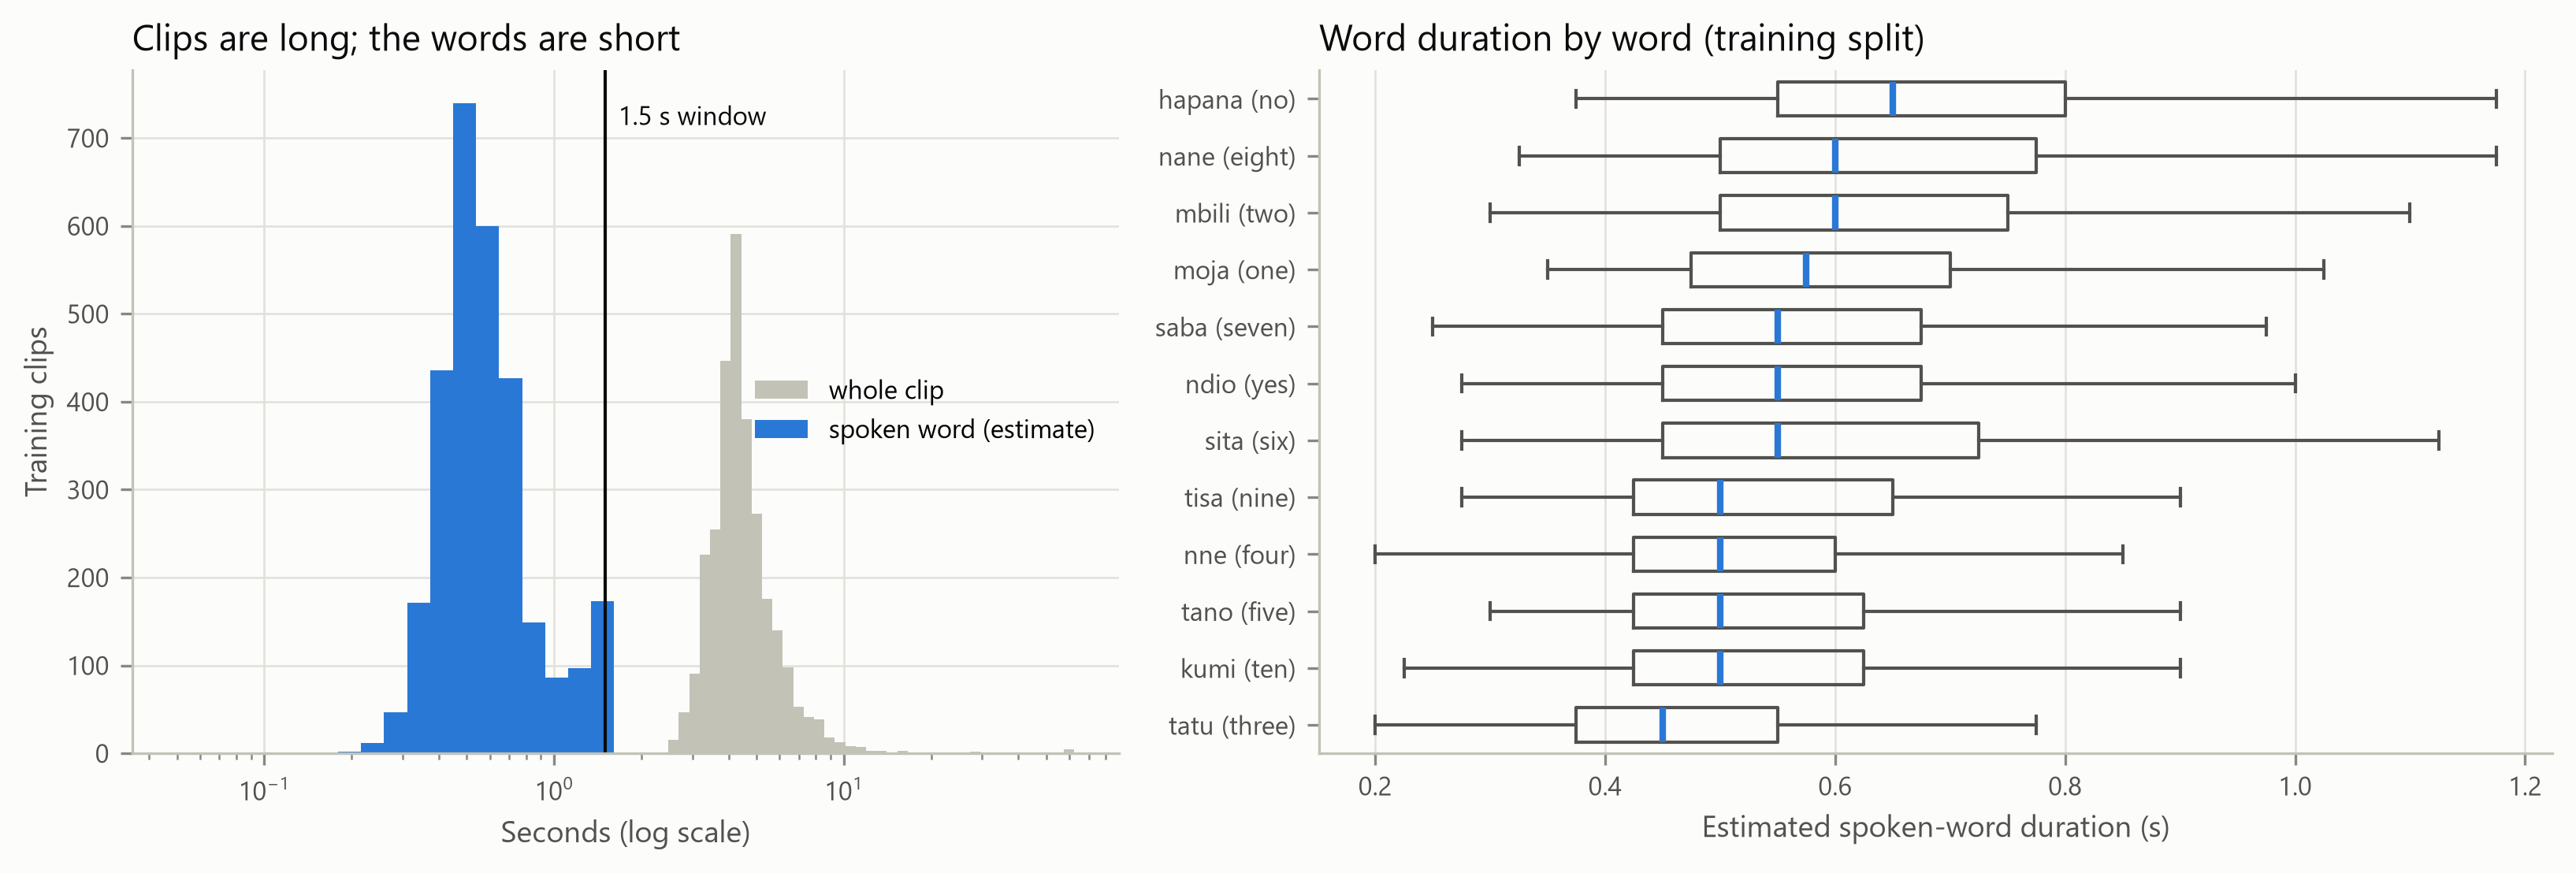
\includegraphics[width=\linewidth]{figures/eda_durations.png}
  \caption{Left: whole clips are far longer than the spoken words they contain (training split, log scale).
  Right: estimated word duration per word.}
  \label{fig:durations}
\end{figure}

\begin{figure}[t]
  \centering
  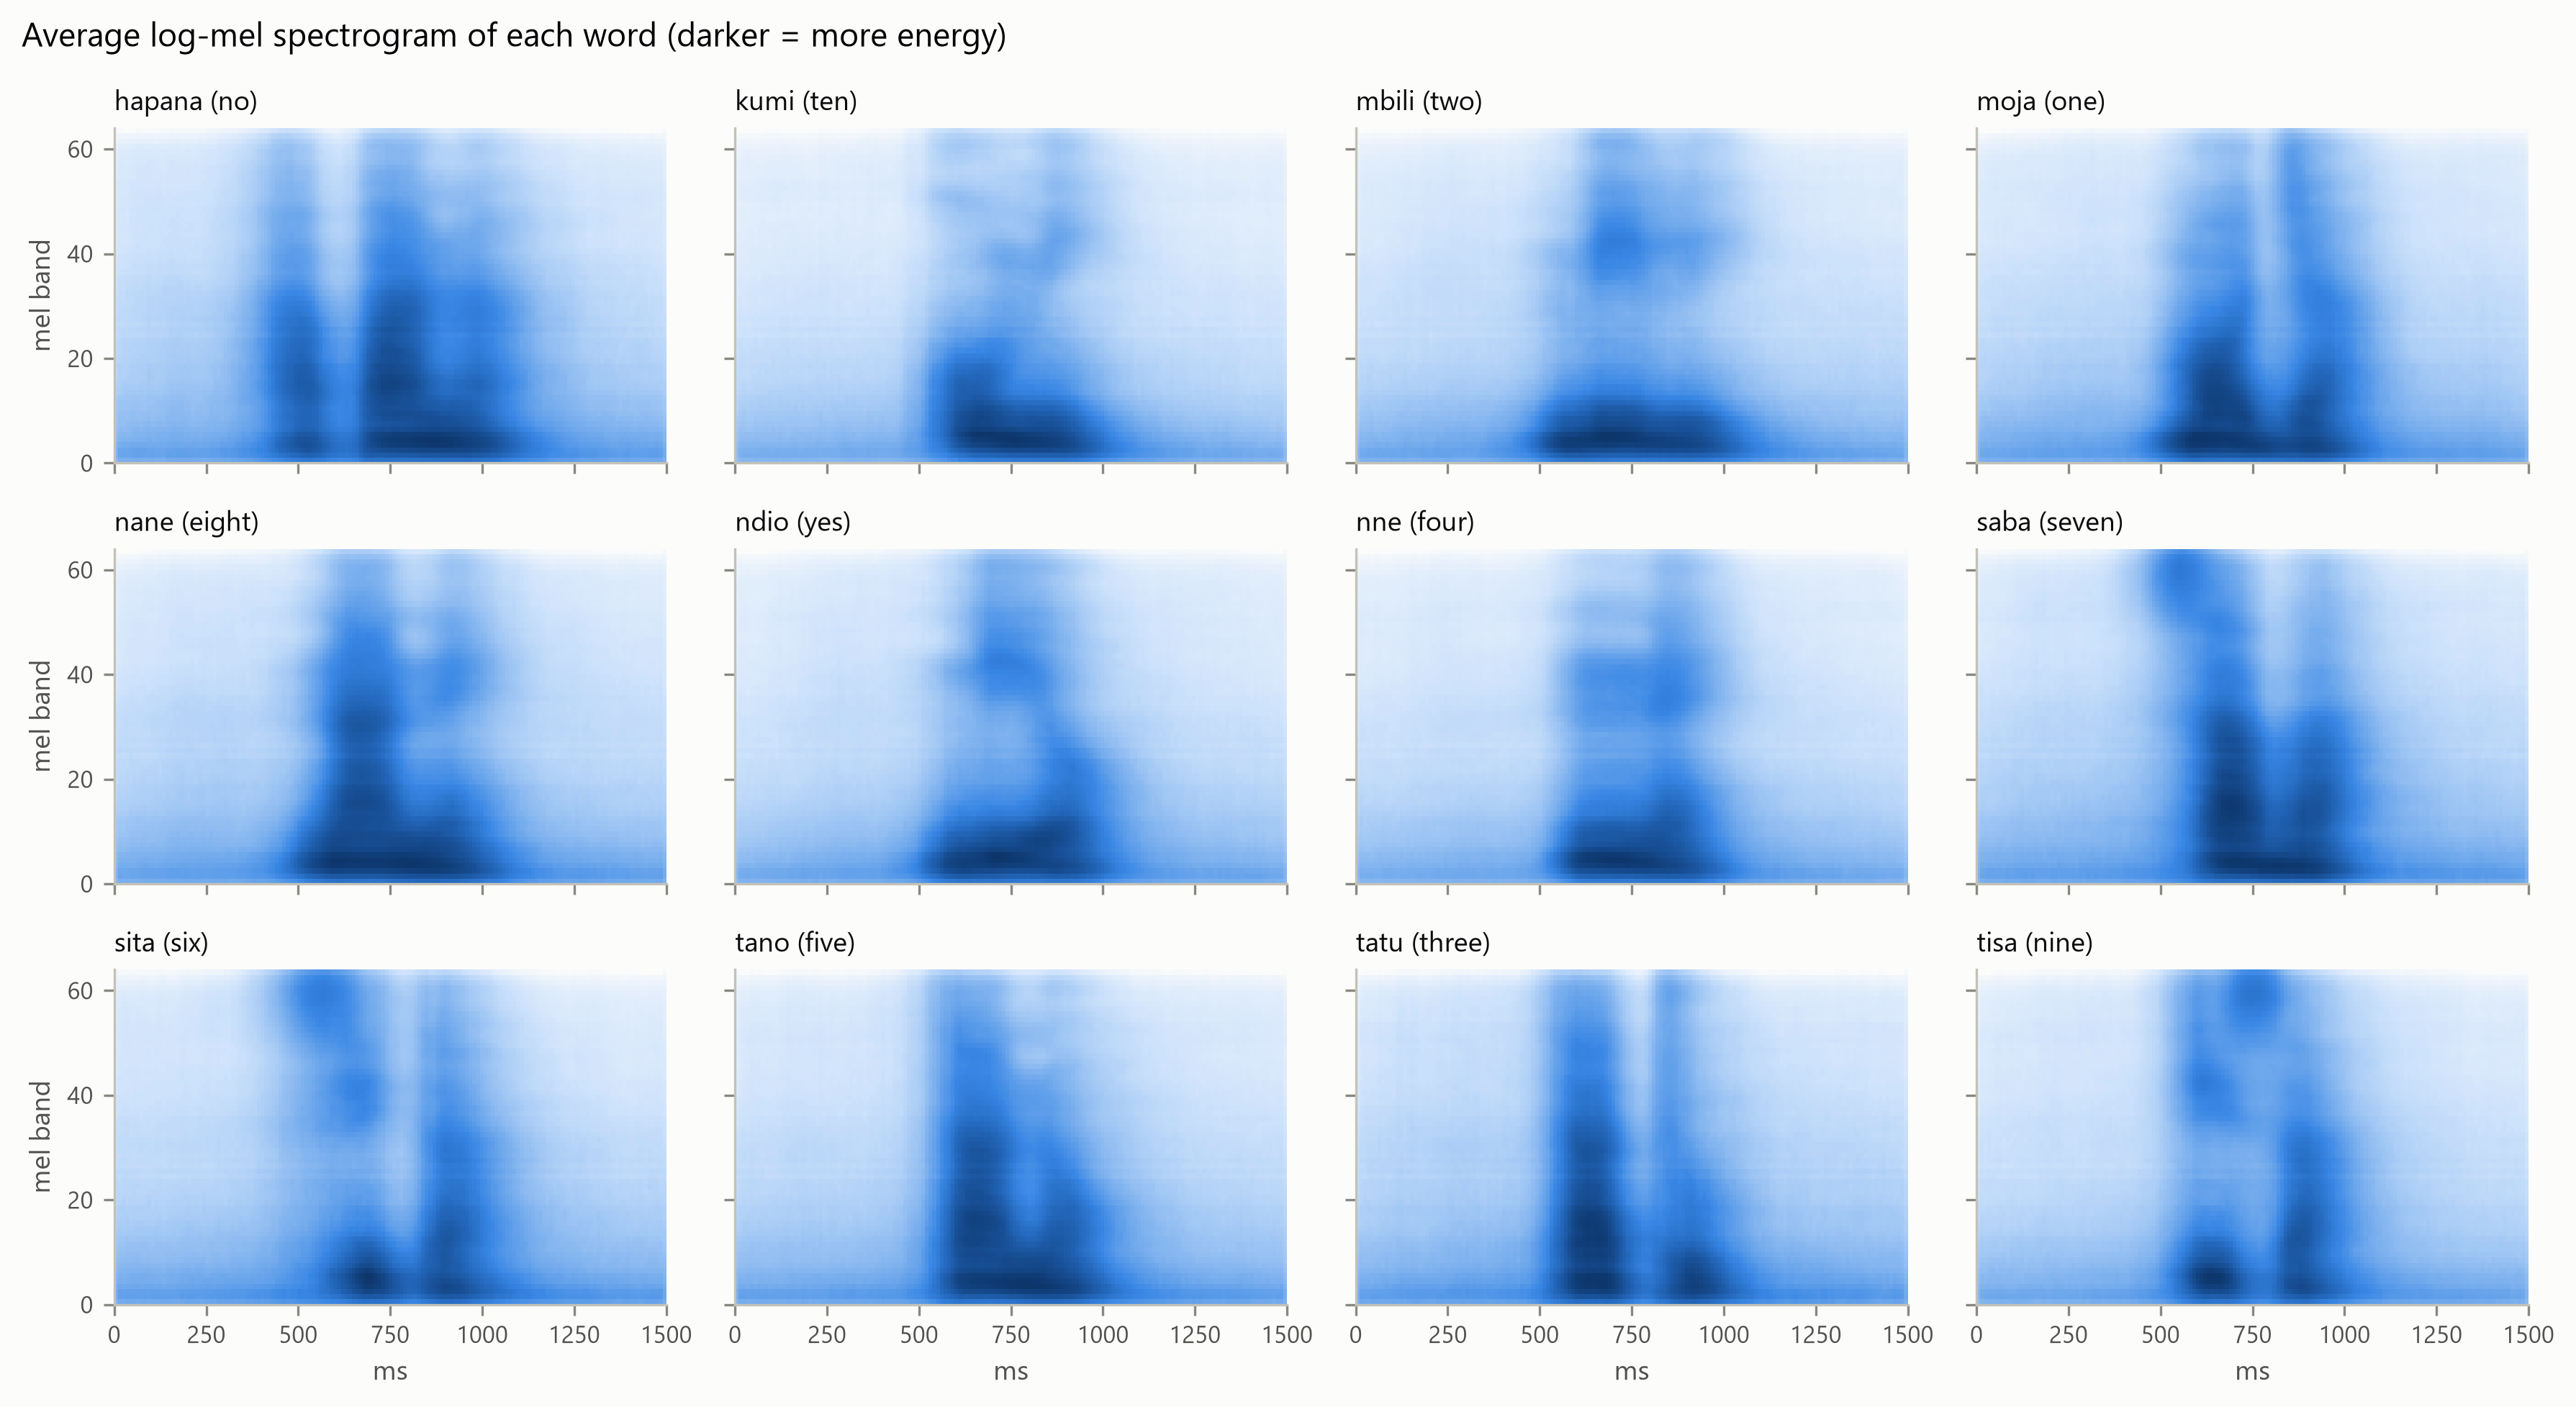
\includegraphics[width=\linewidth]{figures/eda_mean_spectrograms.png}
  \caption{Average log-mel spectrogram of each word in the centred 1.5~s window. The high-frequency /s/ comes at the
  start of \textit{sita} and in the middle of \textit{tisa}.}
  \label{fig:spectra}
\end{figure}

% ---------------------------------------------------------------------------
% Methodology (Section 4) - drafted for M2. The evaluation metrics subsection
% is in evaluation_metrics.tex (M1). Citation keys match report/references.bib.
% Needs in the preamble: \usepackage{booktabs, amsmath}.
% All five approaches are final (A3-A5 configurations in configs/a{3,4,5}_best.yaml).
% ---------------------------------------------------------------------------
\section{Methodology}
\label{sec:method}

\subsection{Data and experimental protocol}
The challenge training set contains 4{,}200 labelled clips (350 per word), all 16~kHz mono 16-bit
PCM~\cite{zindi2021swahili}. The test labels are hidden, so we froze one stratified 70/15/15 split of the training
set (seed 42) into 2{,}940 training, 630 validation and 630 test clips (52--53 per word in validation and test). A
hash of the split is checked by every notebook. No byte-identical duplicate recordings were found.
Model selection uses the validation split only. The test split is scored once, after every configuration is frozen.
Experiments proceed in rounds: R0 establishes each approach, R1 trains default neural configurations, R2 tunes, R3
trains the final configurations with three seeds and evaluates them on the test split, and R4 varies the amount of
training data. Every run is logged with the change it makes and the reason for it (\texttt{results/experiments.csv}).

\subsection{Preprocessing}
Clips last 2.2--62~s (median 4.3~s), but a spoken digit lasts under a second, so most of each clip is silence or
background noise. A single silence-trimming threshold was unreliable: at 30~dB, 10\% of trimmed clips in a
600-clip sample still exceeded 4.5~s. We therefore keep the 1.5~s window with the highest signal energy. When the whole word fits, many
window positions hold almost the same energy, so we take the middle of that plateau. This centres the word: the
energy centroid lies within $\pm0.2$~s of the window centre for 90\% of clips. The window retains a median of
99.8\% of each clip's above-noise energy, and less than 70\% in only 2.7\% of clips, which are mostly long
recordings containing several utterances. Each window is peak-normalised.

\subsection{Acoustic features}
Frames use a 25~ms window and a 10~ms hop, giving 151 frames per window. We compute a 64-band log-mel spectrogram
(dB, 80~dB dynamic range) and mel-frequency cepstral coefficients (MFCCs)~\cite{davis1980comparison} with delta and
delta-delta coefficients (a 9-frame window). Features are computed once, cached, and shared by all members, so every
approach sees identical inputs. Normalisation statistics are always fitted on the training split only.

\subsection{Approaches}
Table~\ref{tab:approaches} summarises the five approaches. They were chosen to vary \emph{how} temporal order is
modelled: not at all (A1), by a generative Markov chain (A2), by recurrence (A3), by convolution over time (A4) and
by self-attention with self-supervised pretraining (A5).

\paragraph{A1: MFCC statistics with a linear classifier}
Each clip becomes one 156-dimensional vector: the mean, standard deviation, minimum and maximum over time of 13
MFCCs with their deltas. This discards temporal order entirely. After standardisation, a multinomial logistic
regression ($C=0.1$, chosen by 5-fold cross-validation on the training split) outperformed an RBF-kernel SVM with
Platt-scaled probabilities~\cite{platt1999probabilistic,wu2004probability}.

\paragraph{A2: GMM-HMM per word}
Following the classic isolated-word recogniser~\cite{rabiner1989tutorial}, each word has its own left-to-right HMM:
each state either repeats or moves to the next. Each state emits diagonal-covariance Gaussian mixtures over
39-dimensional frames (13 MFCCs with deltas). The frames are normalised per utterance (cepstral mean and variance
normalisation, CMVN) to remove the channel differences of about 300 speakers recording on different phones. States
are initialised by a flat start: every training sequence is split uniformly into segments, and state $i$ is
initialised from the $i$-th segments. Training uses Baum--Welch, with small MAP priors on the mixture weights,
variances and allowed transitions. These priors prevent components starved of frames from producing degenerate
(NaN) parameters. A clip is assigned to the word whose model gives the highest per-frame log-likelihood. The final
model has 12 states and 8 Gaussians per state.

\paragraph{A3: bidirectional LSTM with attention}
The log-mel frames ($151\times64$) feed two stacked bidirectional LSTM layers~\cite{hochreiter1997long,graves2013speech}
with 128 units per direction. The outputs are pooled over time with additive attention~\cite{bahdanau2015neural},
followed by dropout and a linear layer over the 12 words. Recurrence carries information across the whole word, and
attention learns which frames matter. It also exposes, for the error analysis, which frames each decision relied on.
The design follows the attention-based recogniser of de Andrade et al.~\cite{deandrade2018neural} with one
deliberate difference. We omit their convolutional layers by default, so that A3 is purely recurrent and contrasts
cleanly with the convolutional A4. Adding them back is one of the R2 ablations.

The R2 search selected:
\begin{itemize}
  \item 40 MFCCs with deltas instead of the log-mel input;
  \item a 1.0~s window;
  \item SpecAugment;
  \item a peak learning rate of $2\times10^{-3}$;
  \item de Andrade et al.'s convolutional front-end (two 1-D convolutions, kernel 5, 128 channels).
\end{itemize}
The final model has 855K parameters. The front-end lowered the validation log loss only marginally ($0.142\to0.134$)
and did not change the accuracy (97.0\%). We therefore also report the purely recurrent variant as the reference
point when comparing recurrence with convolution.

\paragraph{A4: temporal convolutional network (TC-ResNet)}
A4 follows TC-ResNet~\cite{choi2019temporal}. It treats the frequency axis as channels, and slides
one-dimensional convolutions over time only. A three-wide stem convolution feeds residual blocks. Each block has two
convolutions of kernel width 9, the first with stride 2, and a projected shortcut when the shape changes. Global
average pooling over time feeds a linear layer over the 12 words.

Our default is TC-ResNet8 at width 1.5: three blocks with 24--72 channels. It has 146K parameters, and a receptive
field of 171 frames (1.7~s), which already spans the whole input window. Temporal order therefore reaches A4 only
through the arrangement of its strided, stacked filters. There is no state carried through time, as there is in A3.
Because the classifier follows global average pooling, applying it at every time step gives an exact class
activation map over time, which we use for interpretation. The R2 search (below) kept this architecture, and
selected MFCC-40 with $\Delta$ and $\Delta\Delta$ (120 channels) from a 2.0~s window, with full augmentation. The
final model has 150K parameters (\texttt{configs/a4\_best.yaml}), 5.7 times fewer than the final A3.

\paragraph{A5: fine-tuned self-supervised speech transformer}
A5 fine-tunes a Transformer~\cite{vaswani2017attention} speech encoder that was pretrained without labels, following
wav2vec~2.0~\cite{baevski2020wav2vec}. A convolutional feature encoder turns the raw 16~kHz waveform of the same
centred window into one vector per 20~ms. A Transformer then contextualises these vectors, relating every frame to
every other through self-attention. Order enters only through a convolutional positional embedding. The frames of
the last layer are projected to 256 dimensions, mean-pooled over time, and classified.

The default backbone is XLS-R~\cite{babu2022xlsr} with 300M parameters, pretrained on 436K hours in 128 languages,
including 91 hours of Swahili. As is standard, the convolutional feature encoder stays frozen, and the Transformer
is fine-tuned. The new, randomly initialised head has its own, higher learning rate. The only built-in
regularisation is wav2vec~2.0's masking of latent frames: spans of 10 frames, started with probability 0.05. Both
backbones in the R2 comparison use these settings, although they were pretrained with different
defaults. The R2 search kept this setup and added waveform augmentation. The final model has 316M parameters, of
which 311.5M are fine-tuned (\texttt{configs/a5\_best.yaml}): 370 times more than A3 and 2{,}100 times more than A4.

\begin{table}[t]
  \centering
  \caption{The five approaches and how each treats temporal order.}
  \label{tab:approaches}
  \small
  \begin{tabular}{@{}llp{0.42\linewidth}@{}}
    \toprule
    ID & Model & Temporal order \\
    \midrule
    A1 & MFCC statistics + logistic regression & Discarded (bag of frames); $\Delta$ features keep $\sim$90~ms of local change \\
    A2 & GMM-HMM per word & Left-to-right Markov states \\
    A3 & BiLSTM + attention & Recurrence in both directions \\
    A4 & TC-ResNet & Convolution over time \\
    A5 & XLS-R (fine-tuned) & Self-attention; multilingual self-supervised pretraining \\
    \bottomrule
  \end{tabular}
\end{table}

\subsection{Training the neural models}
A3 and A4 share one training loop (\texttt{src/train\_torch.py}):
\begin{itemize}
  \item \emph{Optimisation:} AdamW with a one-cycle learning-rate schedule, gradient clipping at 1.0, cross-entropy
        with label smoothing 0.1, batch size 64, and at most 40 epochs.
  \item \emph{Early stopping:} training stops when the validation log loss (without label smoothing) has not
        improved for five epochs, and the weights of the best epoch are restored.
  \item \emph{Augmentation:} applied on the fly to the feature frames of training clips, using SpecAugment time and
        frequency masking~\cite{park2019specaugment}, time shifts of up to 100~ms and tempo perturbation
        (0.9--1.1$\times$). Noise injection at 10--30~dB SNR assumes a dB power scale, so it is used for log-mel
        inputs only. Padding and masks take the clip's minimum and mean value. For log-mel, whose bands share one
        dB scale, that is one value per clip. A4's MFCC inputs use one value per channel, because their channels
        differ in scale by orders of magnitude. With a single value, the first MFCC run of A4 collapsed to chance.
        All augmentation is synthetic, because the competition allows no external data.
  \item \emph{Reproducibility:} every generator is seeded before the weights are initialised, so a configuration
        reproduces exactly.
\end{itemize}
A5 uses the same loop, instead of a separate fine-tuning framework, so that the loss, model selection and
calibration are identical across the neural models. Four settings differ, as fine-tuning a pretrained model
requires:
\begin{itemize}
  \item each waveform is normalised to zero mean and unit variance inside the model, instead of standardised with
        training-split statistics;
  \item the pretrained Transformer is fine-tuned at a peak learning rate of $3\times10^{-5}$, and the new head at
        $10^{-3}$, with 10\% warm-up;
  \item training runs for 10 epochs with batch 16 and keeps the best epoch, with no early stopping;
  \item augmentation acts on the waveform: time shifts, speed perturbation (0.9--1.1$\times$, which unlike the
        log-mel tempo change also shifts the pitch), and noise at 10--30~dB SNR.
\end{itemize}
Every model's probabilities are then temperature-scaled~\cite{guo2017calibration}, as described in
Section~\ref{sec:metrics}.

\subsection{Hyperparameter search}
Classical models were tuned by grid search: cross-validated on the training split for A1, and on the validation
split for the HMM topology and preprocessing of A2. For A3 we ran a greedy, one-factor-at-a-time search in round R2.
Starting from the default configuration, each run changes a single factor relative to the current best
configuration, and keeps the change only if the validation log loss improves. The factors were augmentation,
pooling (attention, last state, mean), recurrent direction, input features (log-mel or MFCC), window length
(1.0/1.5/2.0~s), the way the word is located, the learning rate, and a convolutional front-end. A4 followed the
same protocol over the factors that apply to it: augmentation, input features, window length, the way the word is
located, depth, kernel width, network width and the learning rate. A5's search covered the pretraining language
(XLS-R against the English-only wav2vec~2.0 Base~\cite{baevski2020wav2vec}), freezing the whole encoder,
augmentation, the window length, a weighted sum of all layers instead of the last~\cite{yang2021superb}, and the
learning rate. This makes every decision traceable to a logged comparison. The cost is that interactions between factors are only explored along the chosen path. Runs that
failed, or that a later fix made stale, are kept outside the results table (\texttt{results/failed\_runs/} and
\texttt{results/superseded\_runs/}).

Single-seed comparisons are noisy, so we measured the noise. Retraining the final A3 configuration with three seeds
(42, 13, 7) gave a validation log loss of $0.137\pm0.004$ (mean $\pm$ SD) and an accuracy of $96.9\pm0.2\%$.
Training is deterministic: the seed-42 run reproduced the R2 result exactly. Search steps that changed the log loss
by about one SD are therefore within seed noise. These include the window length (1.0 versus 1.5~s), the learning
rate and the rejection of the 2.0~s window. We report them, but draw no conclusions from them. Only the larger
effects, such as augmentation, pooling, direction and the way the word is located, are interpreted.

A4 is much less stable across seeds: $0.135\pm0.023$ log loss and $96.8\pm0.3\%$ accuracy. One seed stopped
early, at epoch 16 of 40, while the learning rate was still high. For A4, therefore, only the effect of the way the
word is located (silence trim: $+0.157$ log loss) is clearly larger than seed noise. The other R2 differences
(0.02--0.04) are read as directions, not established effects. A5 is the most stable model: $0.1015\pm0.0009$ log
loss and $98.0\pm0.1\%$ accuracy. Pretrained weights leave the seed little to decide. So all of A5's R2 differences,
except the tie between the 1.5 and 2.0~s windows, are larger than its seed noise.

% TODO: add software references (PyTorch, scikit-learn, librosa, hmmlearn) after verifying them like the others.

% ---------------------------------------------------------------------------
% Evaluation metrics (Methodology, Section 4) - drafted by M1.
% Citation keys match report/references.bib. Numbers come from results/
% (notebooks/02_baselines.ipynb); test-set results are in results_discussion.tex.
% Needs in the preamble: \usepackage{booktabs, amsmath} (table rules, equation).
% ---------------------------------------------------------------------------
\subsection{Evaluation Metrics}
\label{sec:metrics}

The task is closed-set classification of a clip into one of $K=12$ words. Every model outputs a probability
vector $\hat{\mathbf{p}}_i$, and every model is scored by the same code (\texttt{src/evaluate.py}), so the
numbers are comparable across approaches. Table~\ref{tab:metrics} summarises the metrics and what each adds.

\paragraph{Log loss (co-primary)}
The official challenge metric~\cite{zindi2021swahili} is the multi-class log loss,
\begin{equation}
  \mathcal{L} = -\frac{1}{N}\sum_{i=1}^{N} \log \hat{p}_{i,y_i},
\end{equation}
where $y_i$ is the true word of clip $i$. Log loss is a strictly proper scoring rule: its expected value is
minimised only by reporting the true class probabilities, so it rewards honest confidence rather than just the
top-ranked label~\cite{gneiting2007strictly}. This matters for the intended use. A voice interface for mobile
money or a helpline must decide whether to act on a recognised digit or ask the caller to repeat it, and that
decision depends on the confidence. Log loss also punishes confident mistakes severely. Assigning probability
$0.01$ to the true word costs $4.6$ nats, against $\ln 12 \approx 2.48$ for a uniform guess.

Our own experiments show why accuracy alone is not enough. For the MFCC-statistics SVM (an early A1 variant on 40 MFCCs), the probability
method changed the log loss far more than the accuracy. libsvm's pairwise-coupled Platt
probabilities~\cite{platt1999probabilistic,wu2004probability} gave a validation log loss of $0.880$ at $74.3\%$
accuracy. The one-vs-rest sigmoid calibration that scikit-learn now recommends gave $1.230$ at $73.5\%$, and
temperature calibration gave $1.153$ at $73.7\%$. Accuracy is almost unchanged, yet log loss is $40\%$ worse.

\paragraph{Accuracy and macro-F1 (co-primary)}
The training set is exactly balanced (350 clips per word) and the frozen validation and test splits hold 52--53
clips per word. Accuracy is therefore not inflated by a majority class, and it is the conventional headline for
keyword spotting~\cite{warden2018speech}. We also report macro-F1, the unweighted mean of per-class
F1~\cite{sokolova2009systematic}. It penalises a model that over-predicts one word, which accuracy on a balanced
set only partly reveals. We compute it as the mean of per-class F1 scores, not the F1 of mean precision and
recall, since the two definitions can diverge~\cite{opitz2019macro}. Per-class precision, recall and F1, and
the $12\times12$ confusion matrix, show which words fail. For example, A1's recall is only $66\%$ for
\textit{mbili}, which it confuses with \textit{ndio}.

\paragraph{Calibration}
We measure calibration with the expected calibration error (ECE, 15 equal-width confidence
bins)~\cite{naeini2015obtaining,guo2017calibration} and with reliability diagrams. Poor calibration is corrected
post hoc with temperature scaling~\cite{guo2017calibration}: a single scalar $T$ divides the logits (for the
HMM, the per-frame log-likelihoods) before the softmax. It changes the confidence but never the predicted
class, so accuracy and F1 are unaffected. To keep the validation log loss honest, $T$ is \emph{cross-fitted}:
each validation fold is calibrated with a $T$ fitted on the other four folds. $T$ is then refitted on the whole
validation split for use on the test split.

\paragraph{Task-specific diagnostic: sound-alike pairs}
The research question is whether modelling temporal order helps. We therefore track, for word pairs that share
sounds, the share of the pair's clips predicted as the other word of the pair. The pairs are
\textit{tisa}/\textit{sita} (an anagram: the same sounds in a different order), \textit{nne}/\textit{nane},
\textit{tatu}/\textit{tano} and \textit{saba}/\textit{sita}. This links the evaluation directly to the
hypothesis. The order-free A1 confuses \textit{tisa}/\textit{sita} on $6.7\%$ of their validation clips, while
the order-aware HMM (A2) confuses them on none.

\paragraph{Uncertainty and significance}
Model selection uses the validation split only. The test split is used only after every configuration is frozen,
and never for selection. Neural models are trained with three seeds and reported as mean $\pm$ standard
deviation. For every model we compute 95\% percentile bootstrap confidence intervals for accuracy and log loss
(1{,}000 resamples)~\cite{efron1993introduction}; they are listed in \texttt{results/metrics/test\_results.csv}. Pairs of models are compared on the same test clips with the exact
McNemar test on their discordant predictions~\cite{mcnemar1947note}. Dietterich found that this test has an
acceptable Type~I error, and recommends it when each learning algorithm can be run only
once~\cite{dietterich1998approximate}. That fits our setting: retraining the pretrained Transformer the ten
times a $5\times2$ cross-validated test requires is too expensive. The five planned comparisons (the best model
against each other model, and the recurrent A3 against the convolutional A4) are corrected together for
multiplicity with Holm's procedure~\cite{holm1979simple}.

\paragraph{Limitations}
Selection bias, the size of the test split, unknown speakers and the closed vocabulary limit what these metrics can show. They are discussed in Section~\ref{sec:limitations}.

\begin{table}[t]
  \centering
  \caption{Evaluation metrics and their role.}
  \label{tab:metrics}
  \small
  \begin{tabular}{@{}p{0.22\linewidth}p{0.34\linewidth}p{0.34\linewidth}@{}}
    \toprule
    Metric & Why we use it & Limitation \\
    \midrule
    Log loss & Official metric; proper scoring rule; rewards honest confidence & Dominated by a few confident errors \\
    Accuracy & Balanced classes; standard for keyword spotting & Ignores confidence \\
    Macro-F1, per class & Exposes words a model systematically fails & Not a probability metric \\
    ECE + reliability & Directly measures calibration & Depends on binning; sparse bins \\
    Pair confusion & Tests the temporal-order hypothesis & About 105 clips per pair \\
    Bootstrap CI, McNemar & Separates real differences from noise & One split; no speaker grouping \\
    \bottomrule
  \end{tabular}
\end{table}

% ---------------------------------------------------------------------------
% Results and Discussion (Section 5) - drafted for M4.
% Numbers come from notebooks/06_results_error_analysis.ipynb (Parts 1-3) and
% results/metrics/{test_results,test_significance,efficiency,data_size_curve}.csv.
% The main table is generated: results/tables/test_results.tex.
% ---------------------------------------------------------------------------
\section{Results and Discussion}
\label{sec:results}

\subsection{How the configurations were reached}
Table~\ref{tab:ablations} lists the development decisions with the largest effects. It covers 55 logged runs, all
scored on validation.

\emph{Two decisions had the largest effects.} The first is locating the word. Replacing the centred energy window
with silence trimming raised the validation log loss of A3 from 0.144 to 0.759 and of A4 from 0.119 to 0.276. For
the HMM, per-utterance CMVN and the energy window together cut the log loss from 1.65 to 0.38, before any change to
the model. The second, tested on A3, is how the sequence is summarised. A3 with its last hidden state instead of
attention fell from 96.0\% to 69.7\% accuracy, and a forward-only A3 lost 0.09 log loss.

\emph{Augmentation helped every neural model, but in different forms.} SpecAugment gave A3 its largest tuning gain
(0.214 to 0.153), but adding time shift, tempo and noise on top made it worse (0.166). For A4, SpecAugment alone changed
nothing (0.176 to 0.179), while the full set (SpecAugment, time shift, tempo and noise) improved it to 0.140, a gain
of about 1.5 of its seed standard deviations. The waveform counterpart improved A5 (0.111 to 0.101).

\emph{Pretraining needs fine-tuning.} A5 with a frozen encoder reached only 27\% accuracy. English-only
wav2vec~2.0 Base came close to the multilingual XLS-R (0.120 against 0.111), although it is 3.3 times smaller.

\emph{Some differences are within seed noise.} Retraining each final configuration with three seeds gave standard
deviations of 0.004 (A3), 0.023 (A4) and 0.001 (A5) in validation log loss. Differences smaller than these are not
interpreted.

\begin{table*}[t]
  \centering
  \caption{Development decisions with the largest effects (validation log loss, seed 42). Each row changes the
  then-best configuration; the A2 grid and A4's full augmentation change several settings at once. The seed standard
  deviation of the final configurations is 0.004 (A3), 0.023 (A4) and 0.001 (A5).}
  \label{tab:ablations}
  \small
  \begin{tabular}{@{}llrrl@{}}
    \toprule
    Approach & Change & Before & After & Decision \\
    \midrule
    A1 & RBF SVM $\to$ multinomial logistic regression & 0.783 & 0.725 & kept (final) \\
    A1 & 13 $\to$ 40 MFCCs in the statistics & 0.783 & 0.880 & rejected \\
    A2 & + per-utterance CMVN & 1.650 & 0.931 & kept \\
    A2 & silence trim $\to$ centred 1.5~s energy window & 0.931 & 0.380 & kept \\
    A2 & 5 states $\times$ 2 Gaussians $\to$ 12 $\times$ 8 (grid search) & 0.380 & 0.180 & kept (final) \\
    A3 & + SpecAugment & 0.214 & 0.153 & kept \\
    A3 & SpecAugment $\to$ full augmentation & 0.153 & 0.166 & rejected \\
    A3 & attention pooling $\to$ last hidden state & 0.153 & 0.915 & rejected \\
    A3 & bidirectional $\to$ forward-only LSTM & 0.153 & 0.246 & rejected \\
    A3 & energy window $\to$ silence trim & 0.144 & 0.759 & rejected \\
    A3 & + convolutional front-end & 0.142 & 0.134 & kept (final) \\
    A4 & + SpecAugment & 0.176 & 0.179 & rejected \\
    A4 & + full augmentation (SpecAugment, shift, tempo, noise) & 0.176 & 0.140 & kept \\
    A4 & log-mel $\to$ MFCC-40 with deltas (noise then off) & 0.140 & 0.133 & kept \\
    A4 & 1.5~s $\to$ 2.0~s window & 0.133 & 0.119 & kept (final) \\
    A4 & energy window $\to$ silence trim & 0.119 & 0.276 & rejected \\
    A4 & deeper / wider kernels / narrower network & 0.119 & 0.151--0.158 & rejected \\
    A5 & multilingual XLS-R $\to$ English-only wav2vec~2.0 Base & 0.111 & 0.120 & rejected \\
    A5 & fine-tuned $\to$ frozen encoder (head only) & 0.111 & 1.960 & rejected \\
    A5 & + waveform augmentation (shift, speed, noise) & 0.111 & 0.101 & kept (final) \\
    A5 & 1.5~s $\to$ 1.0~s window & 0.101 & 0.130 & rejected \\
    \bottomrule
  \end{tabular}
\end{table*}

\subsection{Test results}
Table~\ref{tab:test} gives the final scores on the 630 test clips. A5 is the best model on
every metric: log loss $0.093\pm0.001$, accuracy $98.1\pm0.1\%$ and macro-F1 0.982 (12 errors for seed 42). A4
follows (log loss 0.125, 96.3\%), then A3 (0.170, 96.0\%), the HMM (0.186, 96.5\%) and the order-free A1 (0.700,
79.5\%).

Validation predicted test well. A5, A2 and A1 moved by at most 0.025 log loss, and A4 improved slightly. A3 lost the
most (0.137 to 0.170). Its configuration combines five search decisions, each chosen on validation, so this is
consistent with selection optimism~\cite{cawley2010overfitting}. With 630 clips, the seed-42 bootstrap intervals
span about $\pm$1--1.5 accuracy points for the order-aware models (for A5, 97.0--99.0\%) and $\pm$3 for A1.

\begin{table*}[t]
  \centering
  \caption{Test results (630 clips; mean $\pm$ SD over three seeds for A3--A5). Params counts all weights. Train is
  the final run's training time (T4 GPU for A3--A5, CPU for A1--A2). CPU ms/clip is the latency
  from audio file to probabilities on one CPU thread.}
  \label{tab:test}
  \small
  \begin{tabular}{@{}lrrrcccc@{}}
\toprule
Approach & Params & Train (min) & CPU ms/clip & Log loss & Accuracy (\%) & Macro-F1 & ECE \\
\midrule
A1 MFCC stats + LR & 2K & 0.1 & 7 & 0.700 & 79.5 & 0.795 & 0.047 \\
A2 GMM-HMM & 93K & 11.0 & 113 & 0.186 & 96.5 & 0.965 & 0.023 \\
A3 BiLSTM + attention & 855K & 1.2 & 14 & 0.170 $\pm$ 0.009 & 96.0 $\pm$ 0.3 & 0.960 $\pm$ 0.003 & 0.017 $\pm$ 0.001 \\
A4 TC-ResNet & 150K & 1.0 & 9 & 0.125 $\pm$ 0.026 & 96.3 $\pm$ 1.2 & 0.963 $\pm$ 0.012 & 0.019 $\pm$ 0.003 \\
A5 XLS-R (fine-tuned) & 316M & 13.0 & 871 & 0.093 $\pm$ 0.001 & 98.1 $\pm$ 0.1 & 0.982 $\pm$ 0.001 & 0.014 $\pm$ 0.003 \\
\bottomrule
\end{tabular}

\end{table*}

\begin{table}[t]
  \centering
  \caption{Significance on the test split (seed 42). McNemar's exact test counts the clips where only one model is
  right; $p$ is Holm-corrected over the five comparisons. $\Delta$ is the difference in log loss (first $-$ second)
  with a paired-bootstrap 95\% interval.}
  \label{tab:significance}
  \footnotesize
  \setlength{\tabcolsep}{3pt}
  \begin{tabular}{@{}lrrrl@{}}
    \toprule
    Comparison & Only 1st & Only 2nd & $p$ & $\Delta$ log loss [95\% CI] \\
    \midrule
    A5 vs A1 & 118 & 1 & $<10^{-32}$ & $-0.608$ [$-0.698$, $-0.531$] \\
    A5 vs A2 & 12 & 2 & 0.039 & $-0.094$ [$-0.133$, $-0.055$] \\
    A5 vs A3 & 13 & 1 & 0.007 & $-0.074$ [$-0.121$, $-0.029$] \\
    A5 vs A4 & 7 & 0 & 0.039 & $-0.014$ [$-0.036$, $+0.005$] \\
    A3 vs A4 & 4 & 9 & 0.27 & $+0.059$ [$+0.018$, $+0.101$] \\
    \bottomrule
  \end{tabular}
\end{table}

\paragraph{Which differences are real}
A5 is significantly more accurate than every other model after Holm's correction (Table~\ref{tab:significance}).
On log loss, its lead over A1--A3 is clear, but its lead over A4 is not: the interval includes zero. A5 makes fewer
errors, while A4's probabilities are nearly as good. The central architectural comparison, recurrence (A3) against
convolution (A4), shows no significant difference in accuracy (4 against 9 discordant clips, $p=0.27$). A4's log
loss is lower, however, by 0.059 [0.018, 0.101]. That holds for seed 42; across seeds the gap (0.170 against 0.125)
is under two of A4's seed standard deviations. The final A3 also has a convolutional front-end, so this compares a
recurrent network with convolutional input layers against a purely convolutional one. The HMM ties with both on
accuracy as well (11 against 9 discordant clips with A3, $p=0.82$; 5 against 8 with A4, $p=0.58$; uncorrected tests
outside the family of Table~\ref{tab:significance}).

\paragraph{Calibration}
Label smoothing leaves every neural model under-confident, and the HMM's raw scores are flatter still (test ECE
0.07--0.23 before scaling). Temperatures fitted on validation (0.38--0.71) transfer to the test split and bring ECE
down to 0.011--0.023.

\paragraph{Where the errors are}
The anagram pair shows the effect of modelling order: \textit{sita}/\textit{tisa} is confused in 8.6\% of its test
clips by A1, but in only 1.0--1.9\% by A2--A5. Per word, A1 fails broadly, while the order-aware models' errors are
spread thinly over many words (Fig.~\ref{fig:perword}). Section~\ref{sec:errors} shows that ten recordings, shared by
all order-aware models, account for 10 of A5's 12 errors and about half of the other models' errors.

\begin{figure}[t]
  \centering
  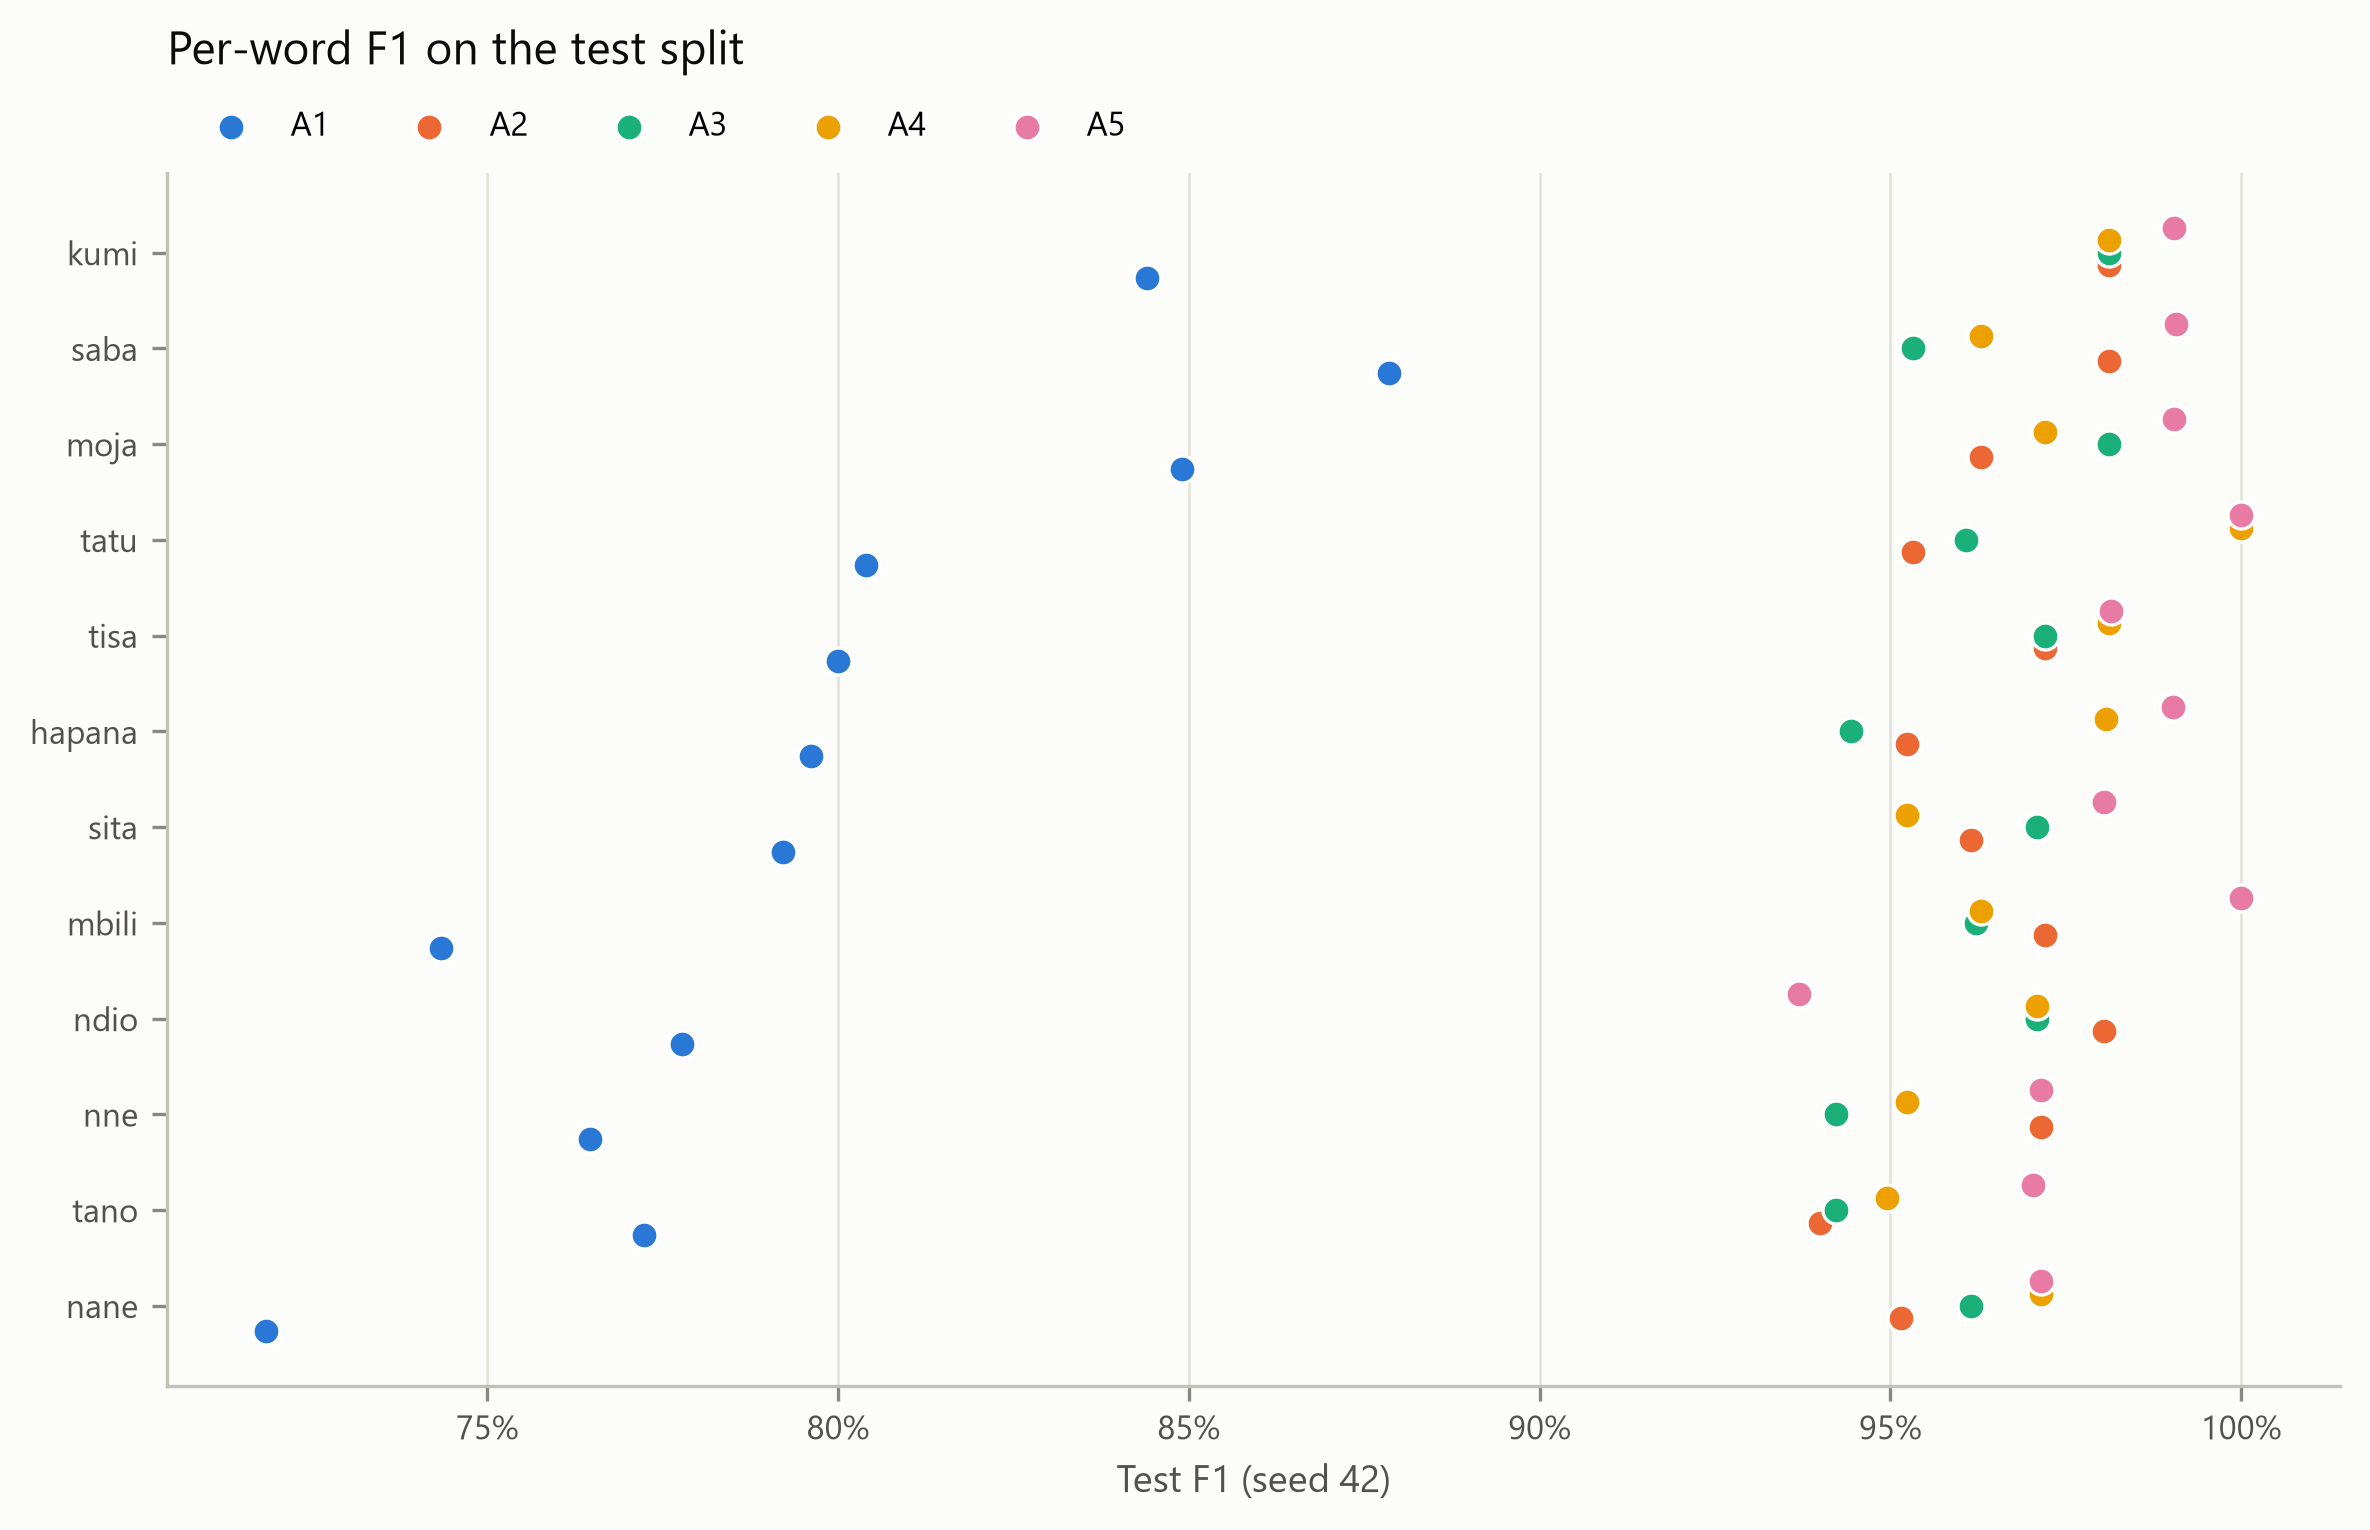
\includegraphics[width=\linewidth]{figures/test_per_word_f1.png}
  \caption{Per-word test F1 (seed 42). The order-free A1 is far behind on every word. The order-aware models stay
  above 93\% on every word.}
  \label{fig:perword}
\end{figure}

\subsection{How much labelled speech is needed}
Each final configuration was retrained on 10, 25 and 50\% of the training clips (nested, stratified subsets; one
seed each) and scored on the test split (Fig.~\ref{fig:datasize}).
\begin{itemize}
  \item \emph{Pretraining pays off most when data is scarce.} With 24 clips per word, A5 reaches 96.5\%. That is about
        as accurate as the models trained from scratch on all 245 clips per word (96.2--97.0\%). It saturates by about
        120 clips per word.
  \item \emph{Without pretraining, the HMM is the most data-efficient model.} At 24 clips per word it reaches
        89.2\%, against 83.5\% for A3 and 62.5\% for A4. From 61 clips per word on, A3 and A4 stay within
        1.4 points of the HMM, and only on the full training set does A4 overtake it.
\end{itemize}
The recipe was held fixed, so the smallest subsets also received fewer optimisation steps. At 10\%, A3--A5 were
still improving at their final epoch, so those points understate them, A4 most of all.

\begin{figure*}[t]
  \centering
  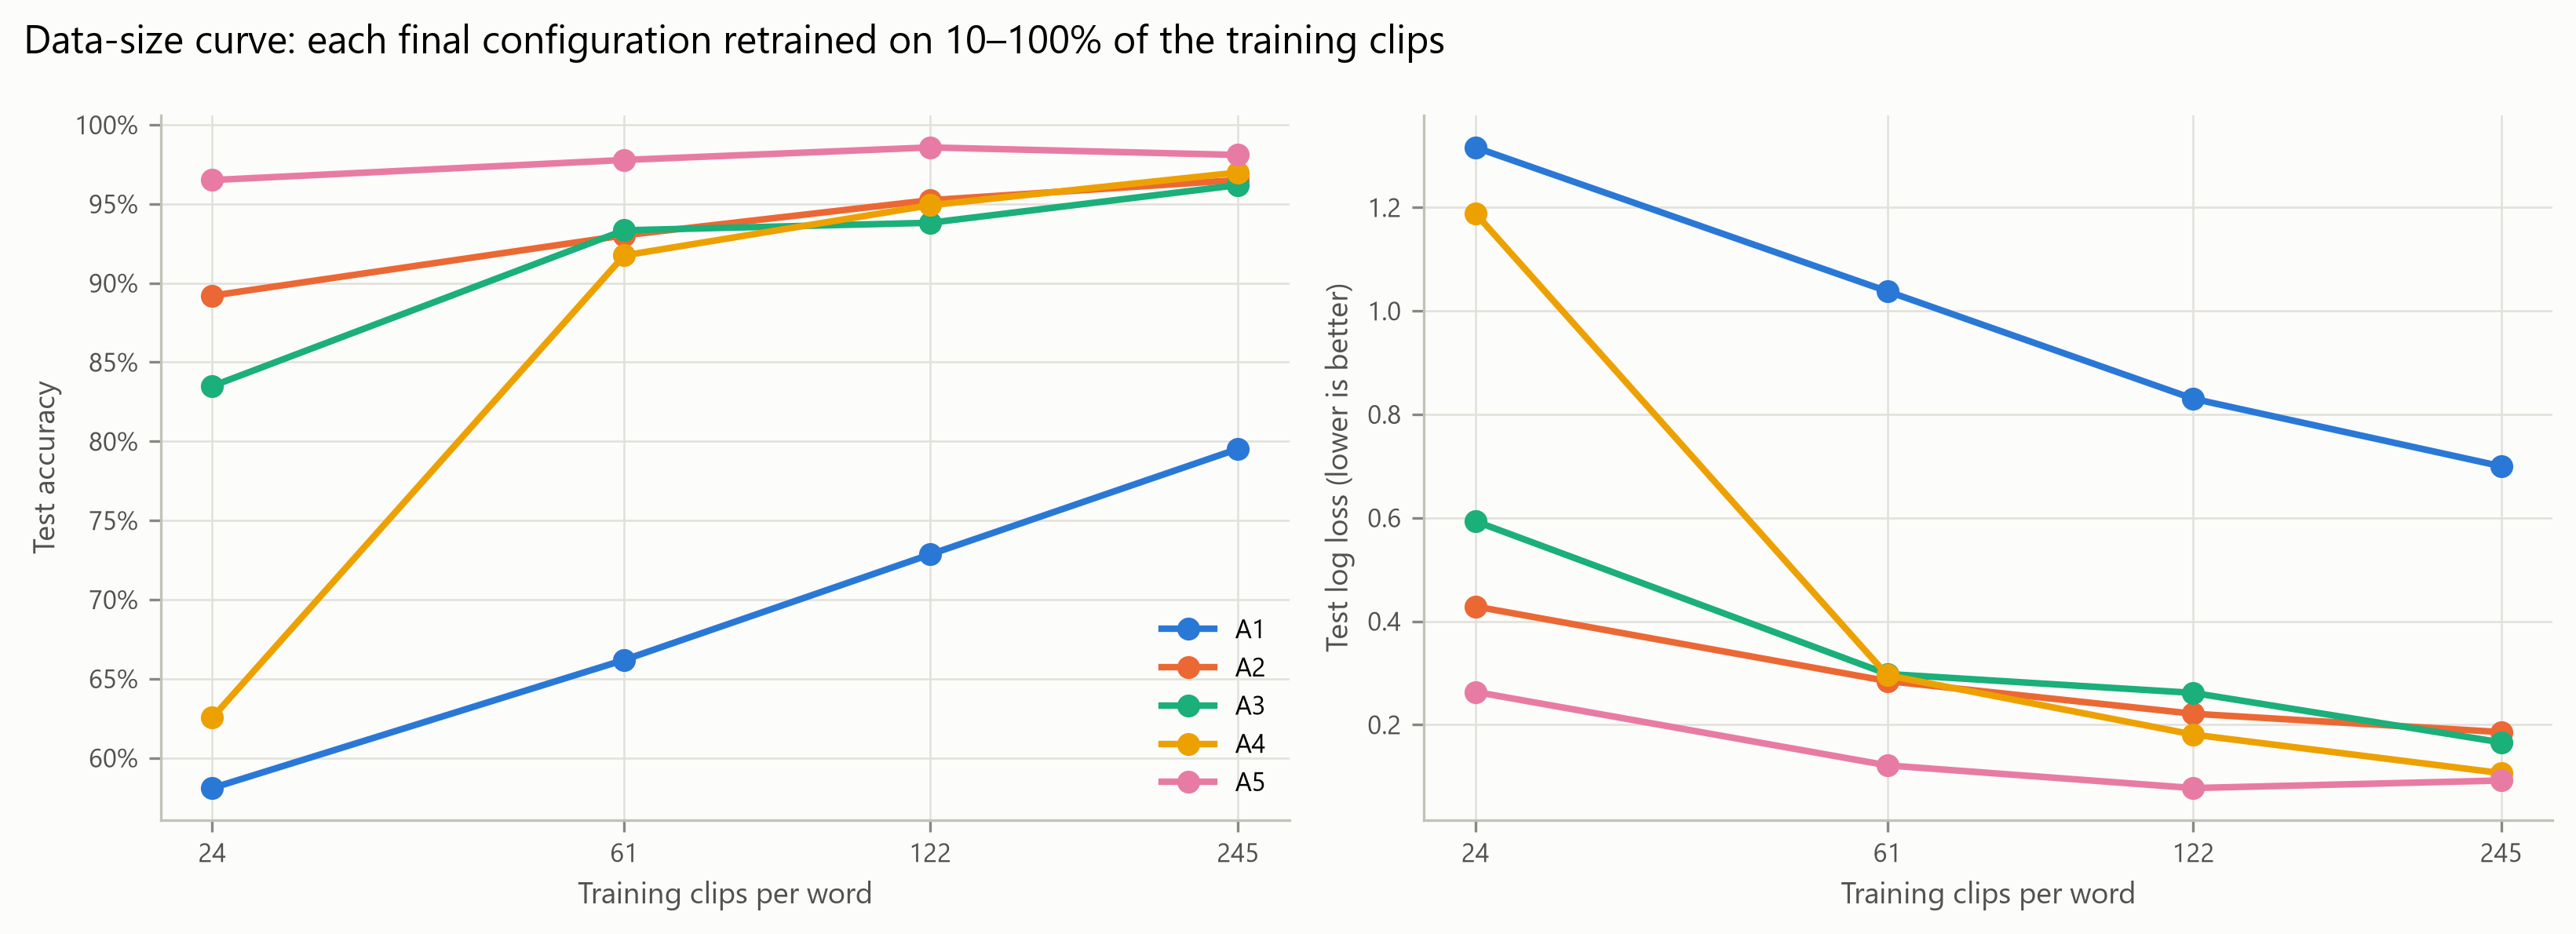
\includegraphics[width=0.78\linewidth]{figures/data_size_curve.png}
  \caption{Test accuracy and log loss when each final configuration is retrained on 10--100\% of the training clips
  (24--245 per word; one seed per point).}
  \label{fig:datasize}
\end{figure*}

\subsection{Cost}
The accuracy has a price (Table~\ref{tab:test}). A5 has 316M parameters (1.26~GB as 32-bit weights) and needs
871~ms per clip on one CPU thread. A4 has 150K parameters (0.6~MB) and needs 9~ms. A5 is thus about 96 times slower and 2{,}100 times
larger, in exchange for 0.032 lower log loss and 1.8 more accuracy points. On a phone or a low-cost voice server, A4
is the efficient choice. Where an error is costly, for example when confirming a mobile-money amount, A5 is worth its
price.

\subsection{Discussion}
We return to the research question: how effectively do sequential models recognise spoken Swahili words, and why?
\begin{enumerate}
  \item \emph{Modelling order is necessary.} Every order-aware model reaches 96--98\% test accuracy, against 79.5\%
        for order-free statistics. A1 also differs in features and capacity, so the gap alone does not prove that
        order is the cause. The anagram pair and the stress test (Section~\ref{sec:errors}) make the link directly,
        as the EDA predicted: the order-aware models confuse \textit{sita} and \textit{tisa} rarely, and fail on
        reversed words. For A5, the order that matters lies mostly within about 100~ms.
  \item \emph{How order is modelled matters less than expected.} A classical HMM ties the neural models trained from
        scratch on accuracy. Convolution matches a BiLSTM with a convolutional front-end in accuracy, with 5.7 times
        fewer parameters, and has a lower log loss for seed 42. This agrees with the finding that convolutional
        networks rival recurrent ones on sequence tasks~\cite{bai2018empirical}, here for sequences as short as a
        single word.
  \item \emph{Pretraining brings the largest gain we observed,} above all with little data. A model that heard only
        91 hours of Swahili during pretraining~\cite{babu2022xlsr}, and an English-only model almost as well,
        transfer effectively to Swahili words. Our design confounds pretraining with A5's architecture, input and
        size (Section~\ref{sec:limitations}), but the result supports self-supervised pretraining as the practical
        route for low-resource languages~\cite{baevski2020wav2vec,doumbouya2021using}.
  \item \emph{The data sets the ceiling.} Locating the word in a long, noisy recording mattered as much as the
        model. Ten test clips defeat every order-aware architecture. They are quiet, noisy or badly cropped far more
        often than other clips, and include a likely label error and words said in English
        (Section~\ref{sec:errors}).
\end{enumerate}

% ---------------------------------------------------------------------------
% Error analysis (Section 6, first part) - drafted for M3 (Phase 8).
% Numbers come from notebooks/06_results_error_analysis.ipynb (Part 4) and
% notebook 07 (order stress test); figures from results/figures/.
% Followed by limitations_responsible_ai.tex. Citation keys match report/references.bib.
% ---------------------------------------------------------------------------
\section{Error Analysis and Limitations}
\label{sec:errors}

\subsection{Error analysis}
The analysis uses the test split and the final seed-42 runs, unless stated otherwise. Confusion rates for A3--A5 are
pooled over their three seeds.

\paragraph{The order-aware models use the order of the sounds}
On the test split, the anagram pair \textit{sita}/\textit{tisa} is the order-free A1's most-confused pair: 8.6\% of
the pair's clips are heard as the other word. For A2--A5 the rate falls to 1.0--1.9\%. Beyond that pair, spelling
similarity does not predict confusion. Across all 66 word pairs, the rank correlation between confusion rate and edit
distance lies between $-0.14$ and $+0.04$ for every model (all $p>0.2$). The closest pair, \textit{nane}/\textit{nne}
(edit distance 1), is confused in 4.7\% of its clips by A1, but in at most 0.3\% by the order-aware models.

The temporal-order stress test (Fig.~\ref{fig:stress}) checks the use of order directly. Each validation clip is
played unchanged, reversed, or cut into 100~ms chunks in random order. Every version keeps the same overall spectral
content, although reversal also reverses the dynamics within each sound, such as a stop's burst.
\begin{itemize}
  \item \emph{Reversal:} accuracy falls from 95--98\% to 21--39\% for A2--A5. On reversed audio, \textit{tisa} is
        mostly heard as \textit{sita} and vice versa: in 83\% of the pair's clips for the HMM and 62\% for A5.
  \item \emph{Control:} a logistic regression on static MFCC statistics alone is exactly unchanged by reversal
        (57.5\%).
  \item \emph{A1:} its delta features encode about 90~ms of local change, so it loses 28 points. It is order-free
        only beyond that scale.
  \item \emph{Shuffling:} A5 keeps 88.9\% accuracy when the chunks are shuffled, while A2--A4 fall to 32--61\%. So
        the pretrained model relies on the order \emph{within} chunks of about 100~ms (the transitions between
        sounds), and hardly on how those pieces are arranged. For the MFCC-based models the comparison is less
        clean, because the cuts also distort their delta features.
\end{itemize}

\begin{figure*}[t]
  \centering
  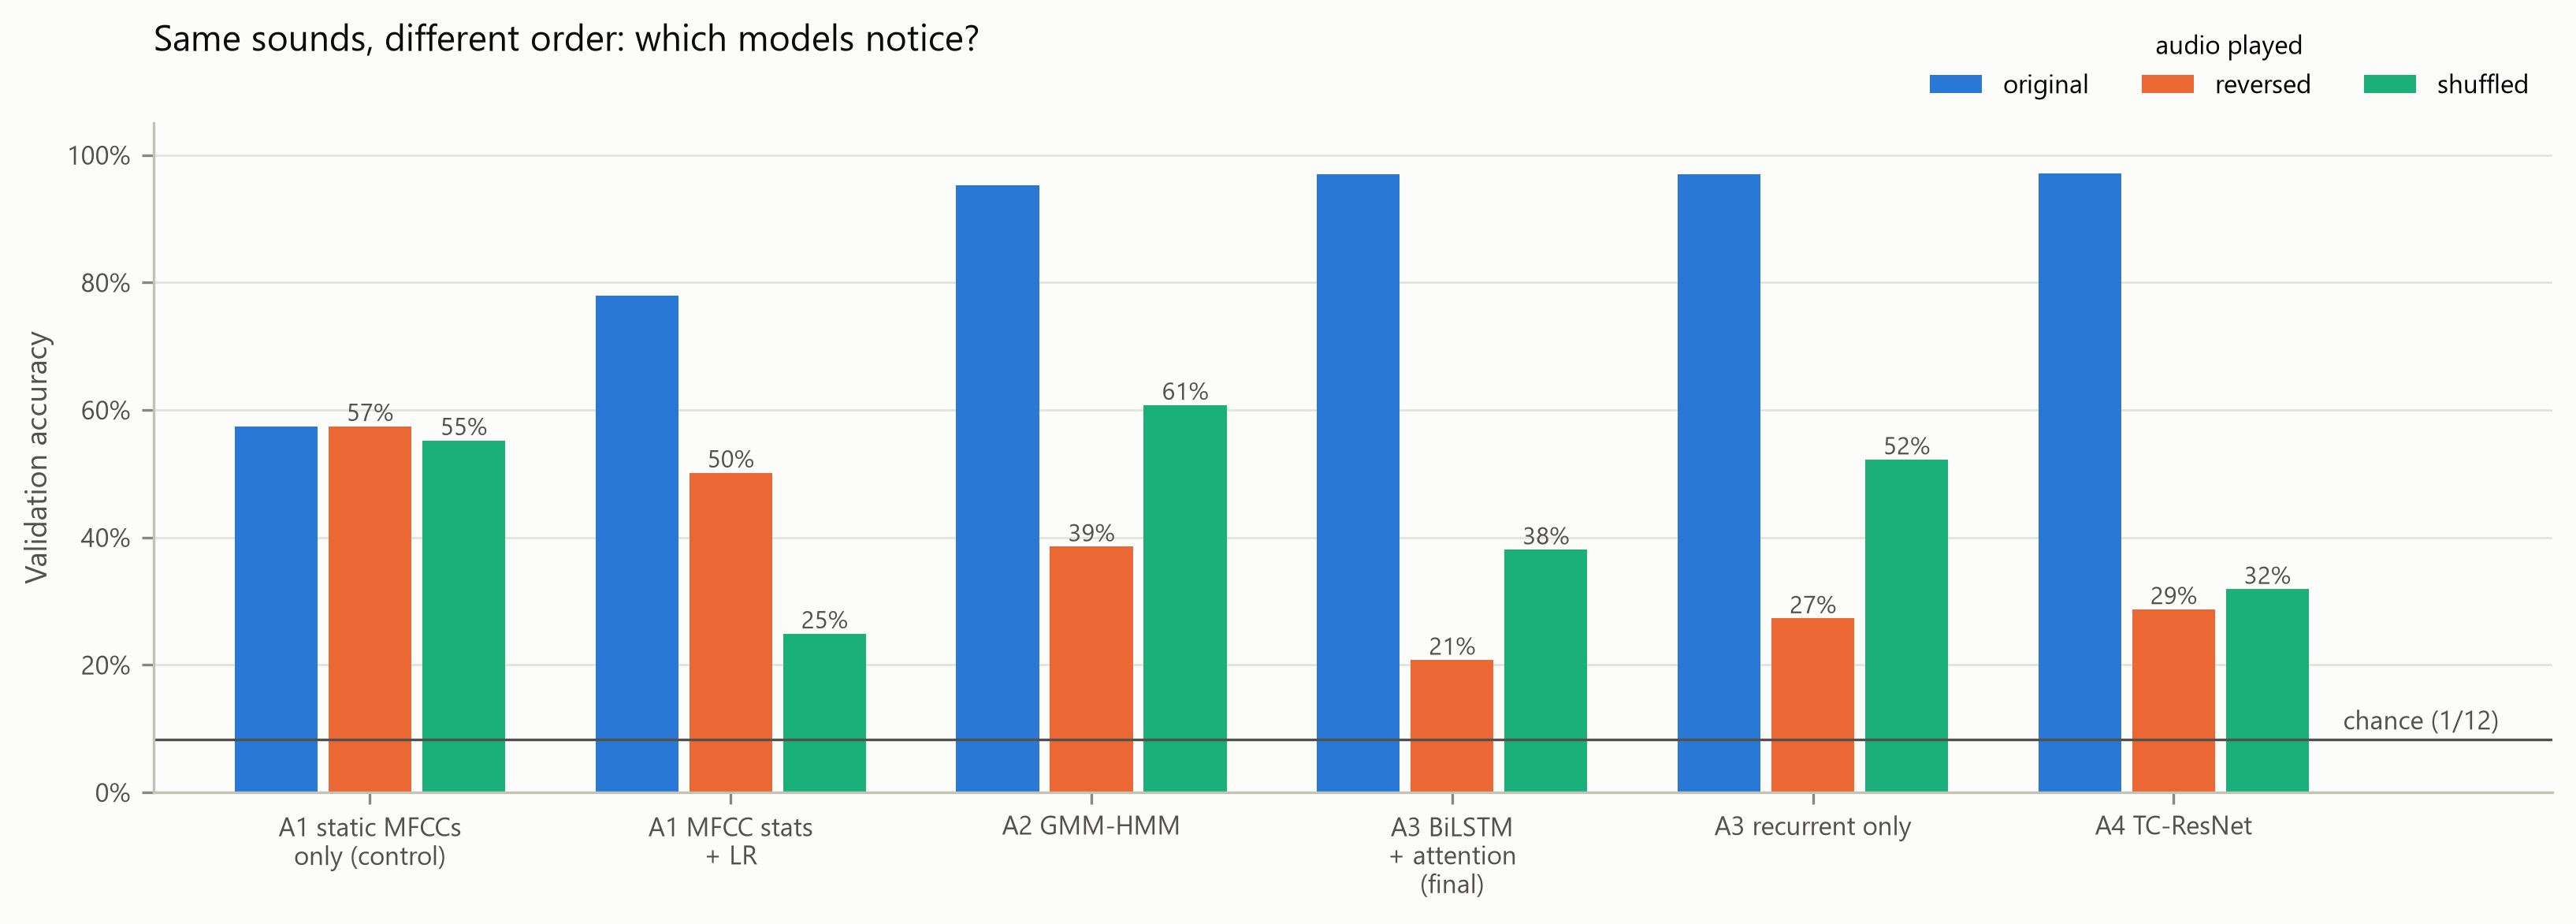
\includegraphics[width=0.78\linewidth]{figures/order_stress_test.png}
  \caption{Validation accuracy when each clip's word is played unchanged, reversed, or as shuffled 100~ms chunks.
  The control is A1 refitted on static MFCC statistics only.}
  \label{fig:stress}
\end{figure*}

\paragraph{The models fail on the same clips}
493 of the 630 test clips (78\%) are recognised by all five models, and 102 defeat only A1. Errors that belong to a
single order-aware architecture are rare: A5 makes none that A2--A4 all avoid, A4 one, A2 seven and A3 eight. The
same 10 test clips defeat A2, A3, A4 and A5 alike. They make up 10 of A5's 12 errors, and 10 of the 19--24 errors
of A2--A4.

Pooling those clips with the 11 validation clips that defeat A2--A5, we compared their recordings with all 1,260
validation and test clips (Table~\ref{tab:hard}).
\begin{itemize}
  \item \emph{Recording problems:} the hard clips are far more often very quiet, contain several separate
        utterances, or have speech at the edge of the default 1.5~s window, which suggests the crop chose the wrong
        stretch. Two-thirds of them are very quiet, noisy or cropped at the edge, against 18\% of all clips.
  \item \emph{Spectrograms:} in about three of the ten hard test clips, the window shows no clear word at all, only
        clicks or near-silence.
  \item \emph{Label-error candidates:} in three clips, A3--A5 agree on the same wrong word with at least 80\%
        confidence. One is a test clip labelled \textit{sita} that all four order-aware models hear as
        \textit{tisa}, with 99--100\% confidence.
\end{itemize}
Agreement among our models is not independent evidence of a label error, because they were all trained on these
labels. We therefore checked the labels in two independent ways.
\begin{itemize}
  \item \emph{Confident learning}~\cite{northcutt2021confident}, applied to the out-of-sample probabilities of A3--A5,
        flags only 1 of the 1,260 validation and test clips: the \textit{sita} clip above.
  \item \emph{An external recogniser:} the multilingual MMS model with its Swahili adapter~\cite{pratap2024scaling},
        which never saw this dataset, transcribed the 21 hard clips. On 60 easy test clips, it finds the labelled
        word in 82\% and never names a wrong one, so its positive findings can be trusted.
\end{itemize}
The recogniser explains six of the hard clips.
\begin{itemize}
  \item \emph{One likely label error:} it hears \textit{tisa} in the clip labelled \textit{sita}, in agreement with
        confident learning and our models.
  \item \emph{Three said in English:} two \textit{hapana} clips contain ``no'', and one \textit{tisa} clip contains
        ``nine''. Our models hear ``nine'' as \textit{nane}.
  \item \emph{Two crop failures:} the labelled word is in the recording, but outside the 1.5~s window.
\end{itemize}
The remaining transcripts contain other speech, such as a different Swahili phrase or English in the background, or
nothing. Because the recogniser also misses the word in 18\% of easy clips, these transcripts are weak evidence on
their own. Six of the 21 hard clips are therefore clear collection problems. For most of the rest, the recording
flags in Table~\ref{tab:hard} point to difficult audio rather than to a weakness of one architecture. Excluding the
two test clips that do not hold the labelled Swahili word raises every model's test accuracy by 0.3 points and leaves
the ranking unchanged. We did not relabel anything.

\begin{table}[t]
  \centering
  \caption{Recording flags among the 21 clips that every order-aware model misclassifies, against all 1,260
  validation and test clips. The window-edge flag uses the default 1.5~s window.}
  \label{tab:hard}
  \small
  \begin{tabular}{@{}lrr@{}}
    \toprule
    Flag & Hard clips & All clips \\
    \midrule
    Very quiet ($<-45$~dBFS) & 38\% & 4\% \\
    Several utterances & 52\% & 25\% \\
    Speech at the window edge & 43\% & 16\% \\
    Low SNR ($<15$~dB) & 14\% & 3\% \\
    Very short ($<0.3$~s of speech) & 10\% & 1\% \\
    Clipped & 0\% & 4\% \\
    \bottomrule
  \end{tabular}
\end{table}

\paragraph{Noise is the main remaining risk}
Error rates rise sharply in noisy recordings (Fig.~\ref{fig:strata}).
\begin{itemize}
  \item \emph{SNR:} below 30~dB (135 test clips), A2--A5 misclassify 8--13\% of clips, against at most 1.5\% above
        30~dB. A5 is the most robust (8.1\%). It is also the only model trained with noise injection, but this
        study cannot separate that from its pretraining.
  \item \emph{Loudness:} quiet recordings are harder for A2--A4 (4.7--8.3\% errors) than for A5 (2.4\%).
  \item \emph{Duration:} words estimated to last over 0.7~s show higher error rates. Part of this is noise
        inflating the estimate: duration and SNR are correlated ($\rho=-0.42$), and among the 50 long clips with good
        SNR, A5 makes one error. A2--A4 still make two or three there (4--6\%), above their overall rates.
\end{itemize}

\begin{figure*}[t]
  \centering
  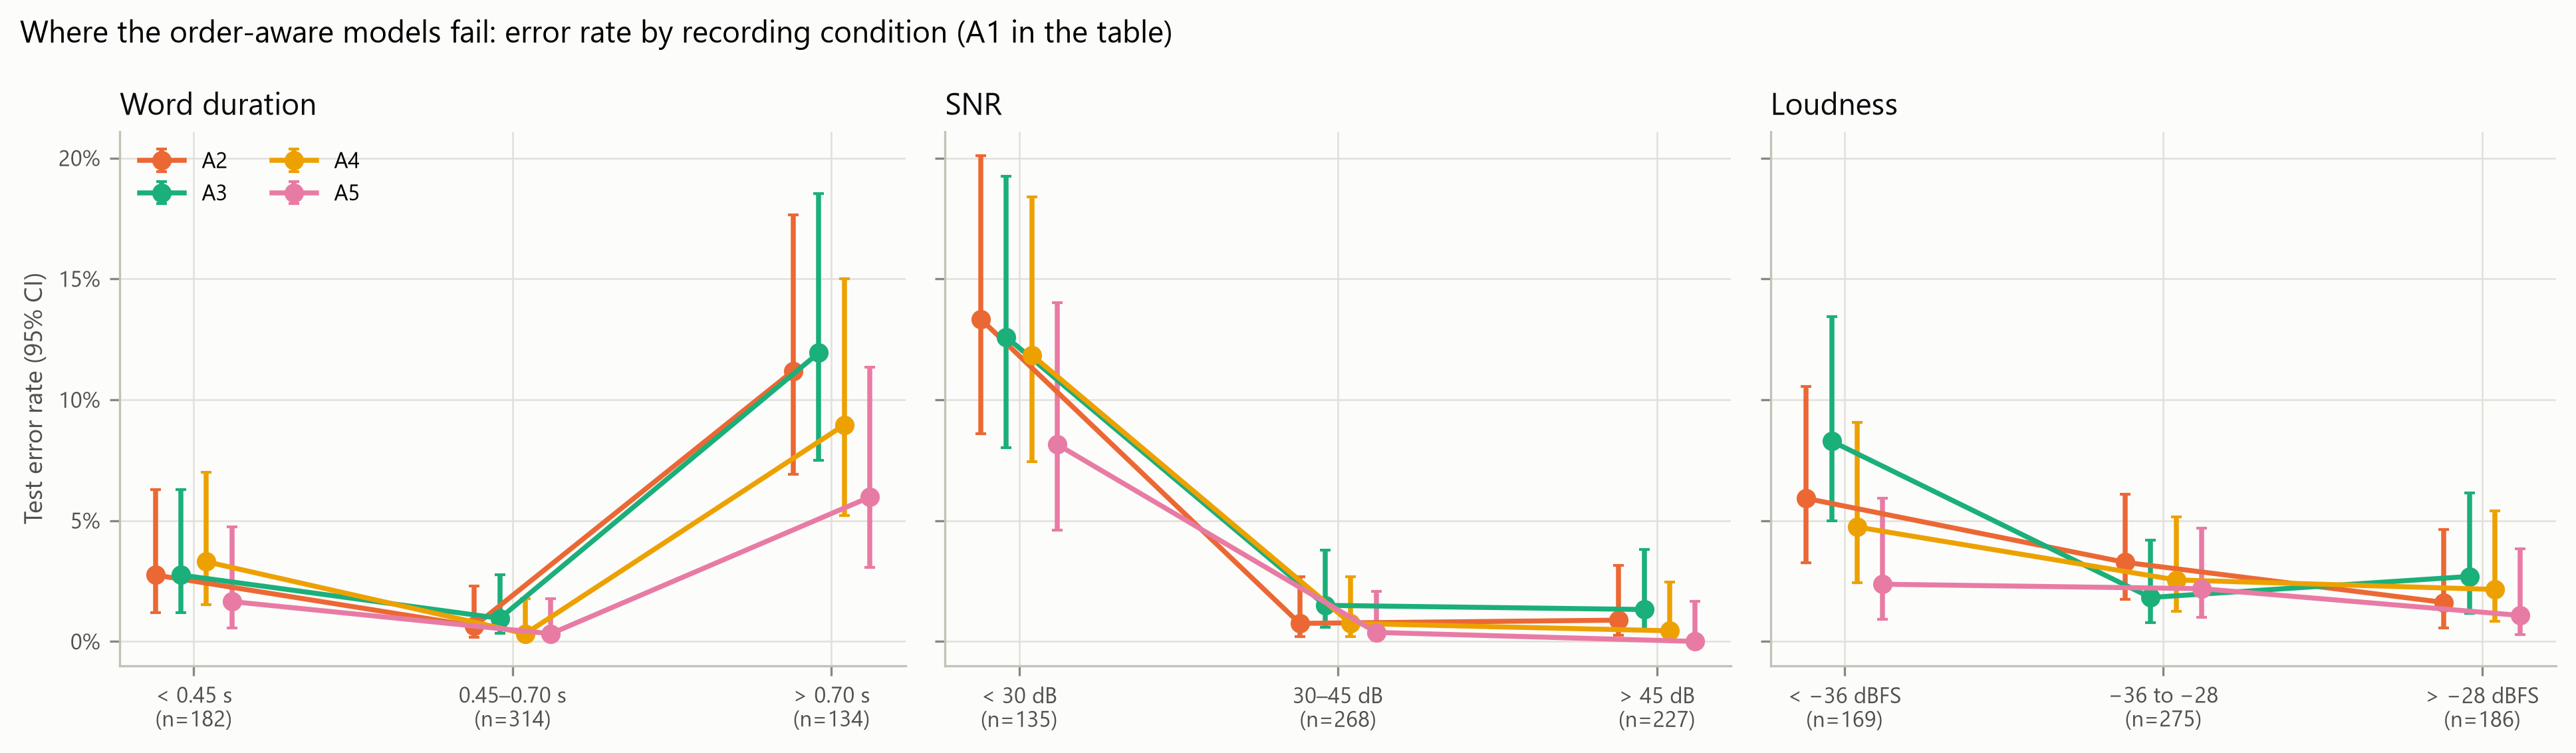
\includegraphics[width=0.82\linewidth]{figures/p8_error_strata.png}
  \caption{Test error rate of the order-aware models by estimated word duration, SNR and loudness, with 95\%
  Wilson intervals.}
  \label{fig:strata}
\end{figure*}

\paragraph{What the models attend to}
\textit{nne} and \textit{nane} differ in the first half of the word, where \textit{nane} has the vowel /a/.
\begin{itemize}
  \item \emph{A3:} its attention peaks about a quarter of the way into both words. The profiles of the two words
        are indistinguishable ($p=0.79$). A bidirectional LSTM summarises the whole word in every state, so the
        attention shows where the model reads its summary, not which sounds decide.
  \item \emph{A4:} its class-activation evidence is spread over the whole word. For \textit{nane} it shifts slightly
        towards the start (56\% against 52\% in the first half, $p=0.014$), as expected if the vowel matters.
  \item \emph{Early recognition:} a forward-only A3 that sees only the beginning of the word reaches 24\% accuracy
        100~ms after the onset, 80\% at 500~ms and 88\% at 800~ms, against 93.7\% for the whole window (validation).
        The evidence separating the confusable words arrives with their second syllable.
\end{itemize}
Perturbation tests such as the stress test give firmer evidence about the use of order than these maps do.

% ---------------------------------------------------------------------------
% Limitations and Responsible AI (part of Section 6) - drafted for M3.
% Follows error_analysis.tex, which opens Section 6 with the Phase 8 analysis.
% Citation keys match report/references.bib.
% ---------------------------------------------------------------------------
\subsection{Limitations}
\label{sec:limitations}
\begin{enumerate}
  \item \emph{Unknown speakers.} The dataset gives no speaker identities, so the frozen split cannot be
        speaker-disjoint. The same person may appear in both training and test clips, and every score may overstate
        performance on new speakers. Keyword-spotting benchmarks usually avoid this by keeping each speaker in one
        partition~\cite{warden2018speech}.
  \item \emph{A closed vocabulary.} Every clip is forced into one of 12 words, and there is no ``unknown word'' or
        ``silence'' class. A deployed system would confidently mislabel anything outside the vocabulary.
  \item \emph{One region, one collection.} All recordings come from crowd-workers in Kenya, collected once. The
        results may not transfer to other varieties of Swahili (for example in Tanzania or the DRC), to other
        recording devices, or to conversational speech.
  \item \emph{Augmentation constrained by the rules.} External data such as noise corpora is not allowed. Our
        synthetic noise (10--30~dB SNR) was harsher than most real clips (median SNR 42~dB), so the augmentation
        study is only a partial test.
  \item \emph{Selection on one validation split.} Configurations were chosen from many validation runs, so
        validation scores are optimistic~\cite{cawley2010overfitting}. Differences of about one seed standard
        deviation (0.004 log loss for A3, 0.023 for A4) are indistinguishable from noise. The test split, never used
        for selection, gives the unbiased estimate.
  \item \emph{Early stopping.} A patience of five epochs stopped one seed each of A3 and A4 at epoch 16 of 40, while
        the learning rate was still high. For A4 that run explains most of the larger seed spread; A3's seeds stayed
        close (0.004). We did not retune the patience after seeing the seed runs, to avoid selecting on validation
        once more.
  \item \emph{Label and collection noise.} 10 test and 11 validation clips defeat every order-aware model. Confident
        learning and an external recogniser identify one likely label error, three words said in English, and two
        recordings where the crop missed the word. For most of the rest the recogniser hears other speech or
        nothing, which is weak evidence on its own (Section~\ref{sec:errors}). No one listened to the clips: our
        evidence is automatic, and the recogniser is itself fallible on short, noisy clips. We did not relabel anything, so these clips count as errors for every
        model. Removing the clear cases changes test accuracy by only 0.3 points.
  \item \emph{Pretraining confounds.} The two A5 backbones differ in size (316M against 95M parameters) as well as
        in pretraining language, and XLS-R's pretraining included only 91 hours of Swahili. A5's gains therefore
        cannot be attributed to Swahili data or to the language of pretraining alone. A Transformer trained from
        scratch, which would separate the architecture from the pretraining, was not run.
  \item \emph{A small test set.} With 630 test clips, accuracy is known to within about $\pm$1--3 points, and
        each sound-alike pair has only about 105 clips.
  \item \emph{Sensitive metrics.} A few confident errors can dominate log loss, so it is always reported with
        accuracy and calibration error. ECE in turn depends on the binning, and its low-confidence bins are sparse.
\end{enumerate}

\subsection{Responsible AI}
\paragraph{Consent and data protection}
Voice recordings are biometric data. The clips were crowdsourced by the challenge organiser under its own terms,
and we honoured its rules: the audio and derived features were never published, were shared only through private
datasets among the group, and are excluded from the public repository.

\paragraph{Fairness we could not measure}
The data carries no speaker metadata (gender, age, dialect or region), so we could not test whether error rates
differ between groups. The wide pitch range suggests a mix of voices, but that is no substitute for a fairness
audit. Speakers of other Swahili varieties, children and older adults may be served worse by any model trained
only on these recordings.

What we could measure is recording conditions, and they matter. In noisy recordings (SNR below 30~dB), the
order-aware models make 8--13\% errors, against at most 1.5\% in cleaner ones (Section~\ref{sec:errors}). Users
with cheap phones or in noisy places, often the same users that spoken interfaces aim to include, would therefore
see several times more errors than the headline accuracy suggests.

\paragraph{Consequences of errors}
The intended applications, such as spoken digits for mobile money, helplines or menu navigation for users with
limited literacy~\cite{doumbouya2021using}, turn a misrecognised digit into a wrong transaction or a wrong service.
Calibration therefore matters as much as accuracy. A deployed system should confirm uncertain inputs, which is why
we report log loss and calibration error, and why we apply temperature scaling. Because the vocabulary is closed,
it also needs a way to reject speech outside the vocabulary.

\paragraph{Dual use}
Keyword spotting in under-resourced African languages has humanitarian uses, such as monitoring radio for relief
programmes~\cite{menon2018fast}. The same technology could also be used for surveillance of speech. The models
here recognise only 12 isolated words, which limits that risk.

\paragraph{Environmental cost}
The neural models were trained on one Kaggle Tesla~T4, except one A4 run on a laptop CPU; the classical models ran
on CPUs. All 19 logged A3 runs took about 10 minutes of GPU time in total. All of A4's runs, including the failed
and superseded ones, took under 30 minutes. The pretrained A5 dominates the budget: its 16 runs, including one failed
run and the three data-size runs, took about 2.8 hours. That is about 11 minutes per run, against about one minute
or less for A3 and A4. Even so, the compute and energy cost of the study is small, and we fine-tuned the smallest
XLS-R model rather than the 1B or 2B versions.

\paragraph{Use of AI assistance}
We used AI to plan the project and to help us understand some complex situations.

% ---------------------------------------------------------------------------
% Conclusion and Future Work (Section 7).
% ---------------------------------------------------------------------------
\section{Conclusion and Future Work}
\label{sec:conclusion}

We asked how effectively sequential models recognise spoken Swahili words. On 12 crowdsourced Swahili words they do
so very effectively, and the evidence points to three findings and one limit.
\begin{itemize}
  \item \emph{Order:} the order-aware models reach 96--98\% accuracy, against 79.5\% for order-free statistics. The
        models also differ in capacity, but the anagram pair and the stress test show that every order-aware model
        depends on order.
  \item \emph{The kind of sequence model} matters less than expected. A classical HMM, a BiLSTM and a TC-ResNet reach
        similar accuracy. The convolutional model has the lowest log loss of the three (seed 42; within two seed
        standard deviations across seeds), with under a fifth of the BiLSTM's parameters.
  \item \emph{Pretraining} brings the largest gain we observed, although our design cannot separate it from A5's
        architecture and size. The fine-tuned XLS-R is the best and most stable model (98.1\% test accuracy, log
        loss 0.093). With 24 clips per word it is about as accurate as the models trained from scratch on ten times
        more data. The price is 96 times the latency and 2{,}100 times the size of A4.
  \item \emph{The limit is the data.} The clips that defeat every order-aware model are mostly quiet, noisy or badly
        cropped, and include a likely label error and words said in English. Noise is the main risk for deployment.
\end{itemize}

\paragraph{Future work}
\begin{itemize}
  \item \emph{Speaker-disjoint evaluation:} cluster speaker embeddings into pseudo-speakers, to measure how much
        speaker overlap inflates our scores.
  \item \emph{Noise robustness:} multi-condition training with realistic noise, where the rules allow it, since
        errors concentrate below 30~dB SNR.
  \item \emph{Rejecting other speech:} an ``unknown'' and ``silence'' class, and voice-activity detection, to avoid
        the crop failures and to reject words outside the vocabulary.
  \item \emph{Separating architecture from pretraining:} a Transformer trained from scratch~\cite{berg2021keyword},
        and a backbone covering more African languages (MMS~\cite{pratap2024scaling}).
  \item \emph{Deployment:} distilling A5 into an A4-sized model for phones, and streaming recognition, for which a
        forward-only recurrent model already reaches 80\% accuracy 500~ms into the word.
\end{itemize}


\section*{Team and Contributions}
Ownership followed the project plan: \MemberOne{} (M1) the data pipeline, evaluation and baselines A1--A2; \MemberTwo{} (M2) augmentation, the training loop and A3; \MemberThree{} (M3) the EDA, A4 and the error analysis; \MemberFour{} (M4) A5 and the final evaluation. Commits and tasks per member are in the contribution tracker.

\section*{AI-Use Statement}
AI was used extensively to plan the project, to understand complex scenarios, and to help write some of the codes.

\bibliographystyle{IEEEtran}
\bibliography{references}

\end{document}
